% dimer.tex — Chapter 3: Dimer BSSE Analysis
% Project: rmrresearch/bsse_db | Branch: fcuantico
% Molecules: Ne (complete), H2O (complete), HF (placeholder)

% ======================================================================
\section{Ne Dimer}
% ======================================================================

% ----------------------------------------------------------------------
\subsection{Overview}
% ----------------------------------------------------------------------

The Ne dimer serves as the simplest baseline case in this study. Neon
is a noble gas with a spherically symmetric electron density, so the
BSSE between two Ne monomers is expected to depend only on their
separation distance, with no orientational dependence. This makes the
Ne dimer an ideal system for isolating the purely radial behavior of
BSSE before introducing the geometric complexity of polyatomic
molecules. All calculations were performed at the SCF, MP2, and
CCSD(T) levels using the aug-cc-pVDZ basis set~\cite{dunning1989,kendall1992}
for the translational scan and aug-cc-pVTZ for the radial scan, with
the NWChem quantum chemistry package~\cite{nwchem2020}.

The BSSE for each dimer configuration is computed as:
\begin{equation}
    \Theta_{AB}(AB) = \Delta E_{AB}(A, B, AB) - \Delta E_{AB}(AB)
    \label{eq:ne_dimer_bsse}
\end{equation}
where $\Delta E_{AB}(A, B, AB) = E_{AB}(AB) - E_A(A) - E_B(B)$ is the
uncorrected interaction energy and $\Delta E_{AB}(AB) = E_{AB}(AB) -
E_A(AB) - E_B(AB)$ is the Boys--Bernardi counterpoise-corrected
interaction energy~\cite{boys1970}. Energies are reported in Hartree
and distances in \AA.

% ----------------------------------------------------------------------
\subsection{Experimental Design}
% ----------------------------------------------------------------------

In the translational scan, monomer A (Ne) is fixed at the origin and
monomer B (Ne) is displaced along a three-dimensional grid. The scan
is organized into fixed-$y$ slices; only the slices at $y = 1.5$ and
$y = \SI{1.75}{\angstrom}$ form complete $7 \times 7$ grids (49 points
each) and are used for contour analysis. The displacement components
are varied in increments of \SI{0.25}{\angstrom}, and the axes of each
contour plot correspond to the in-plane Ne--Ne displacement components
$(x, z)$ in \AA.

Because Ne is a spherically symmetric atom, no rotational scan was
performed: rotating a Ne monomer about any axis produces an identical
configuration. The translational scan therefore constitutes the
complete characterization of the Ne dimer BSSE anisotropy.

% ----------------------------------------------------------------------
\subsection{Translational Scan Results}
% ----------------------------------------------------------------------

Figure~\ref{fig:ne_trnl_contours} shows the BSSE contour plots for the
fixed-$y$ slices at $y = 1.5$ and \SI{1.75}{\angstrom} for all three
levels of theory. Each panel shows BSSE as a function of the in-plane
Ne--Ne displacement components $(x, z)$.

\begin{figure}[!ht]
    \centering
    \begin{subfigure}[b]{0.32\textwidth}
        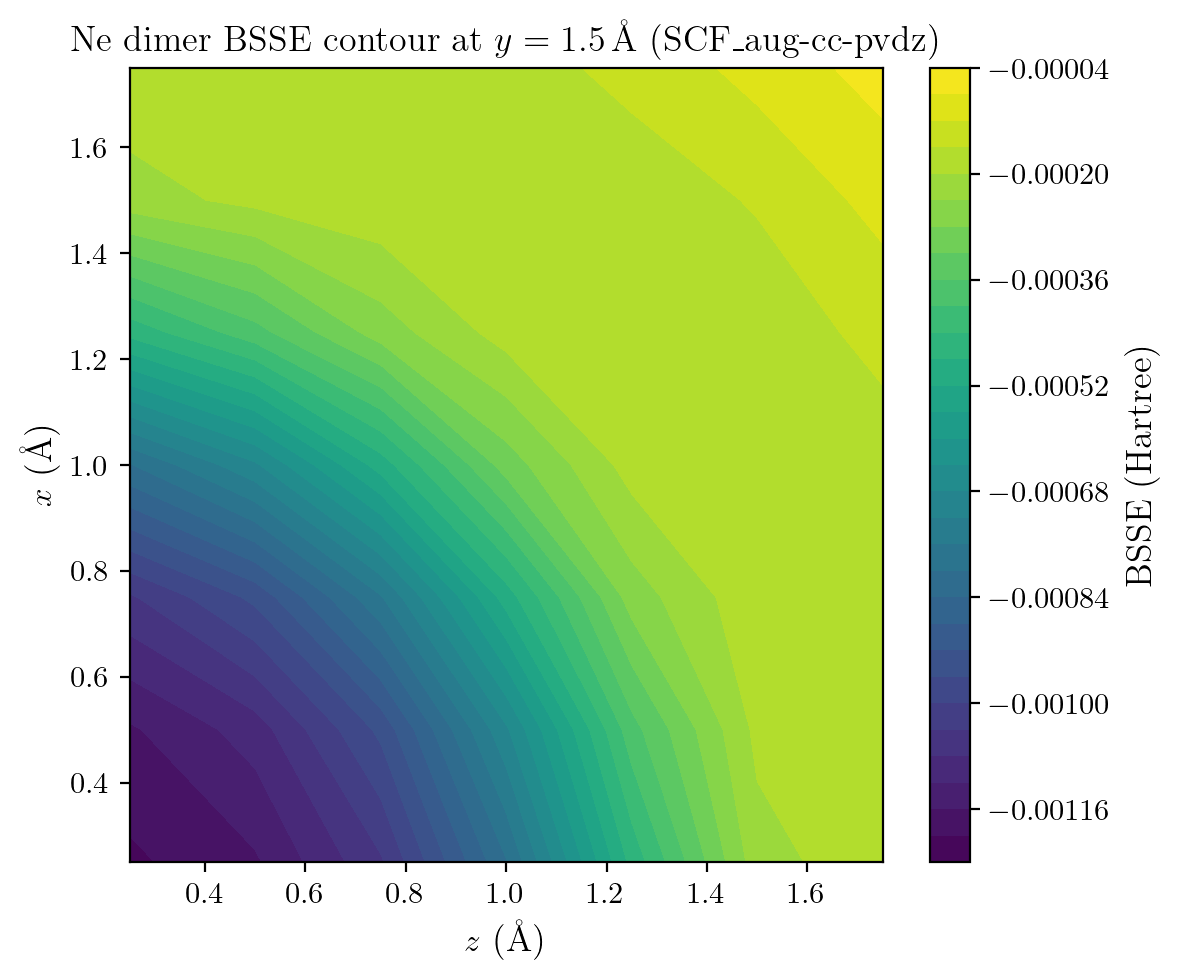
\includegraphics[width=\textwidth]{figures/dimer/Ne_dimer/Ne_trnl_contour_1.5_SCF.png}
        \caption{SCF, $y = \SI{1.5}{\angstrom}$}
    \end{subfigure}
    \hfill
    \begin{subfigure}[b]{0.32\textwidth}
        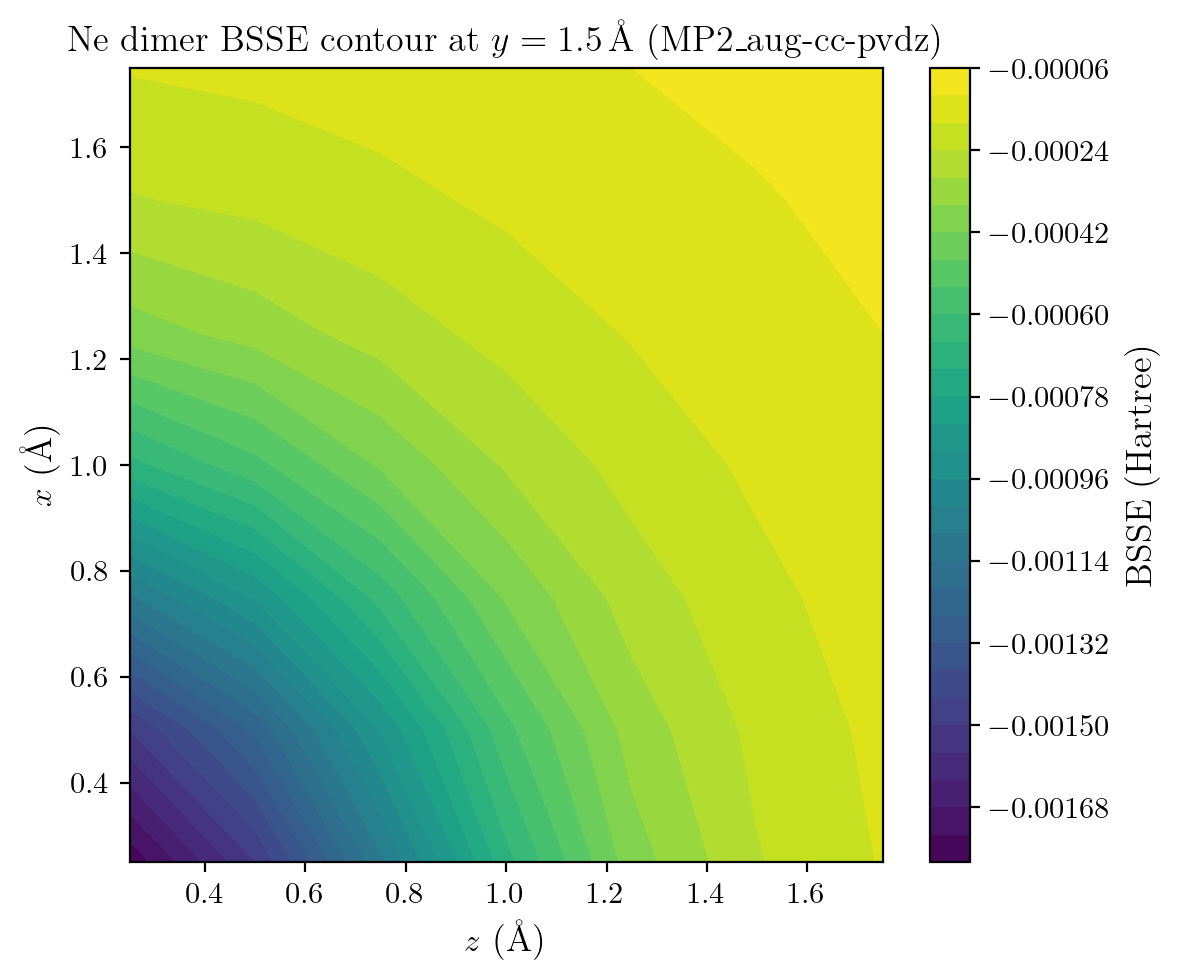
\includegraphics[width=\textwidth]{figures/dimer/Ne_dimer/Ne_trnl_contour_1.5_MP2.png}
        \caption{MP2 corr., $y = \SI{1.5}{\angstrom}$}
    \end{subfigure}
    \hfill
    \begin{subfigure}[b]{0.32\textwidth}
        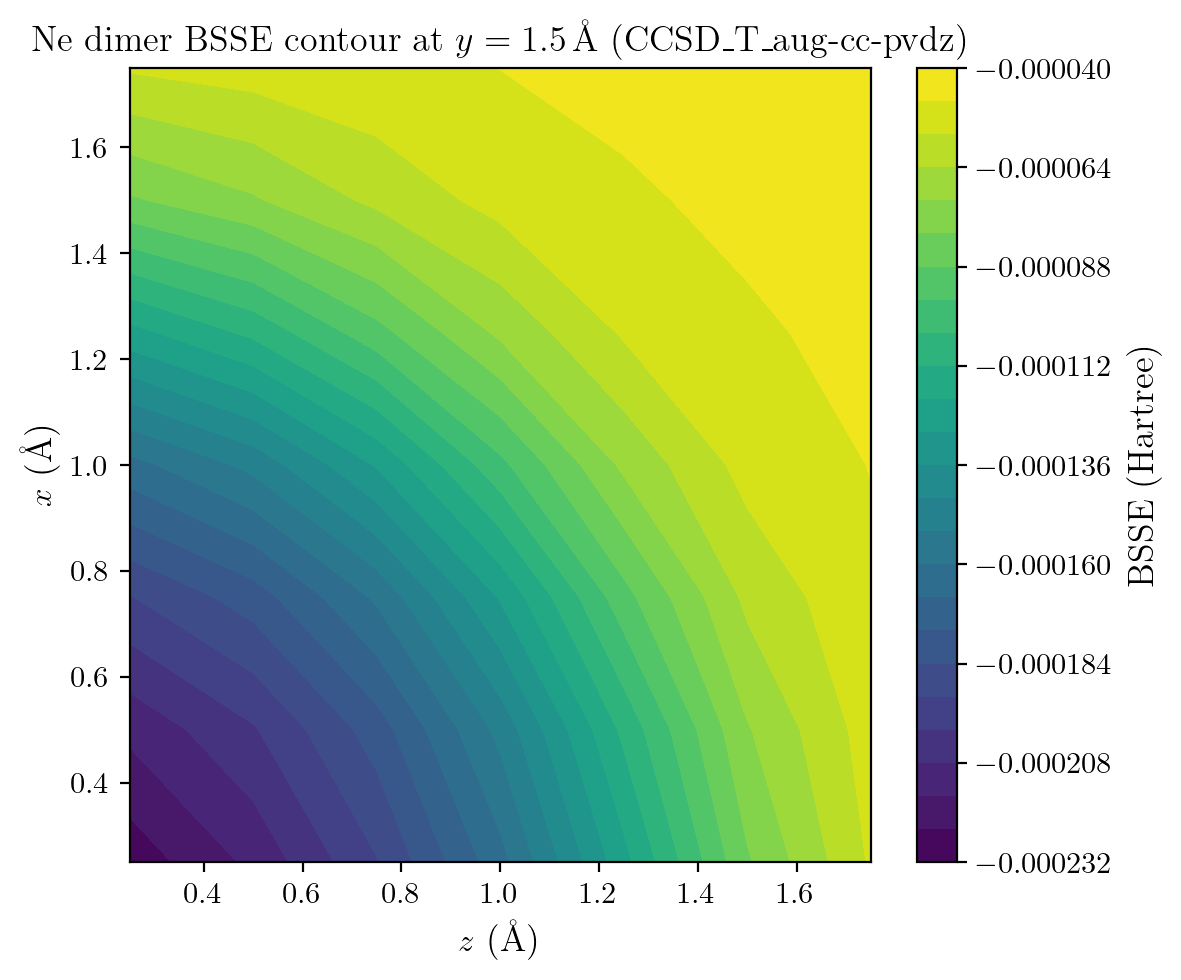
\includegraphics[width=\textwidth]{figures/dimer/Ne_dimer/Ne_trnl_contour_1.5_CCSD_T.png}
        \caption{CCSD(T) corr., $y = \SI{1.5}{\angstrom}$}
    \end{subfigure}

    \vspace{0.8em}

    \begin{subfigure}[b]{0.32\textwidth}
        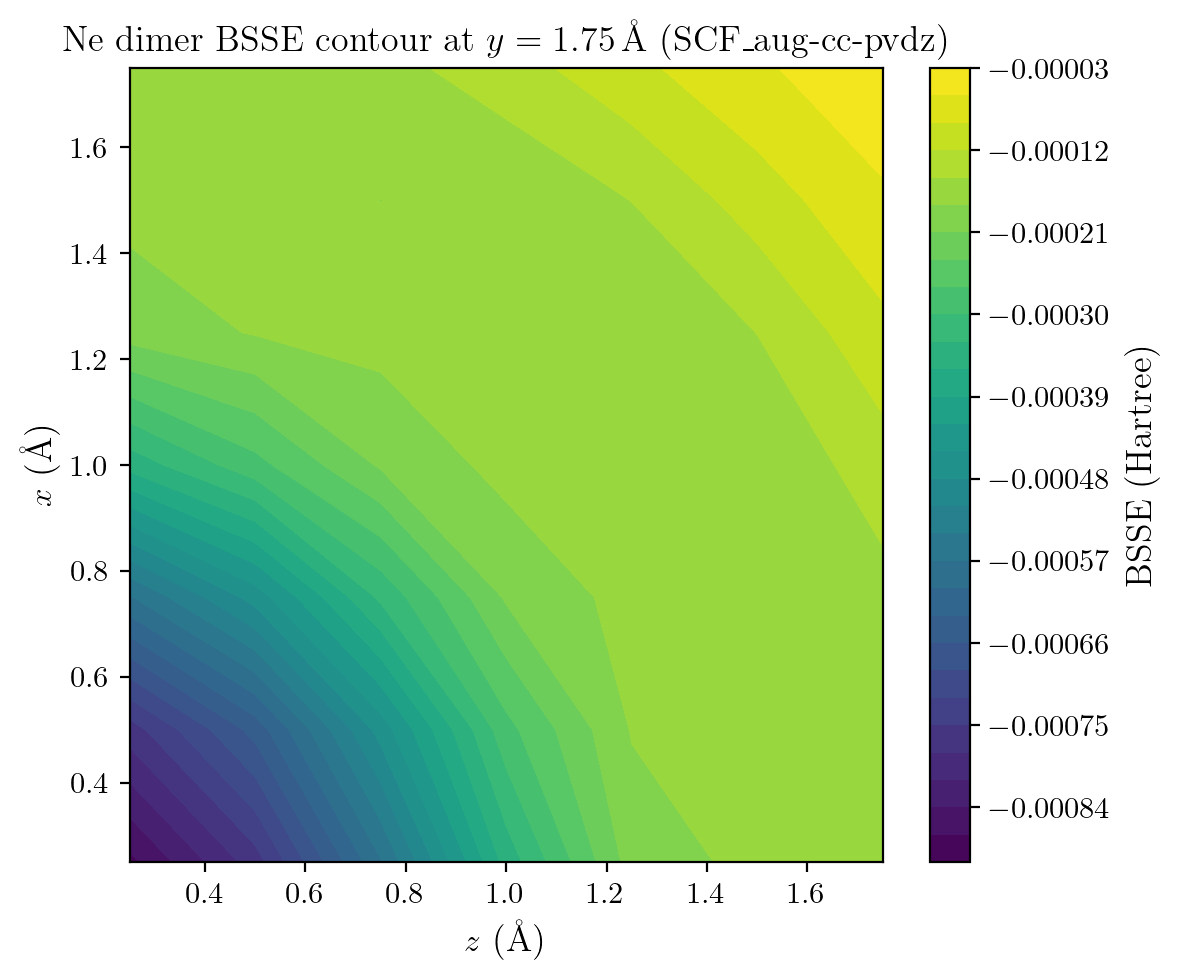
\includegraphics[width=\textwidth]{figures/dimer/Ne_dimer/Ne_trnl_contour_1.75_SCF.png}
        \caption{SCF, $y = \SI{1.75}{\angstrom}$}
    \end{subfigure}
    \hfill
    \begin{subfigure}[b]{0.32\textwidth}
        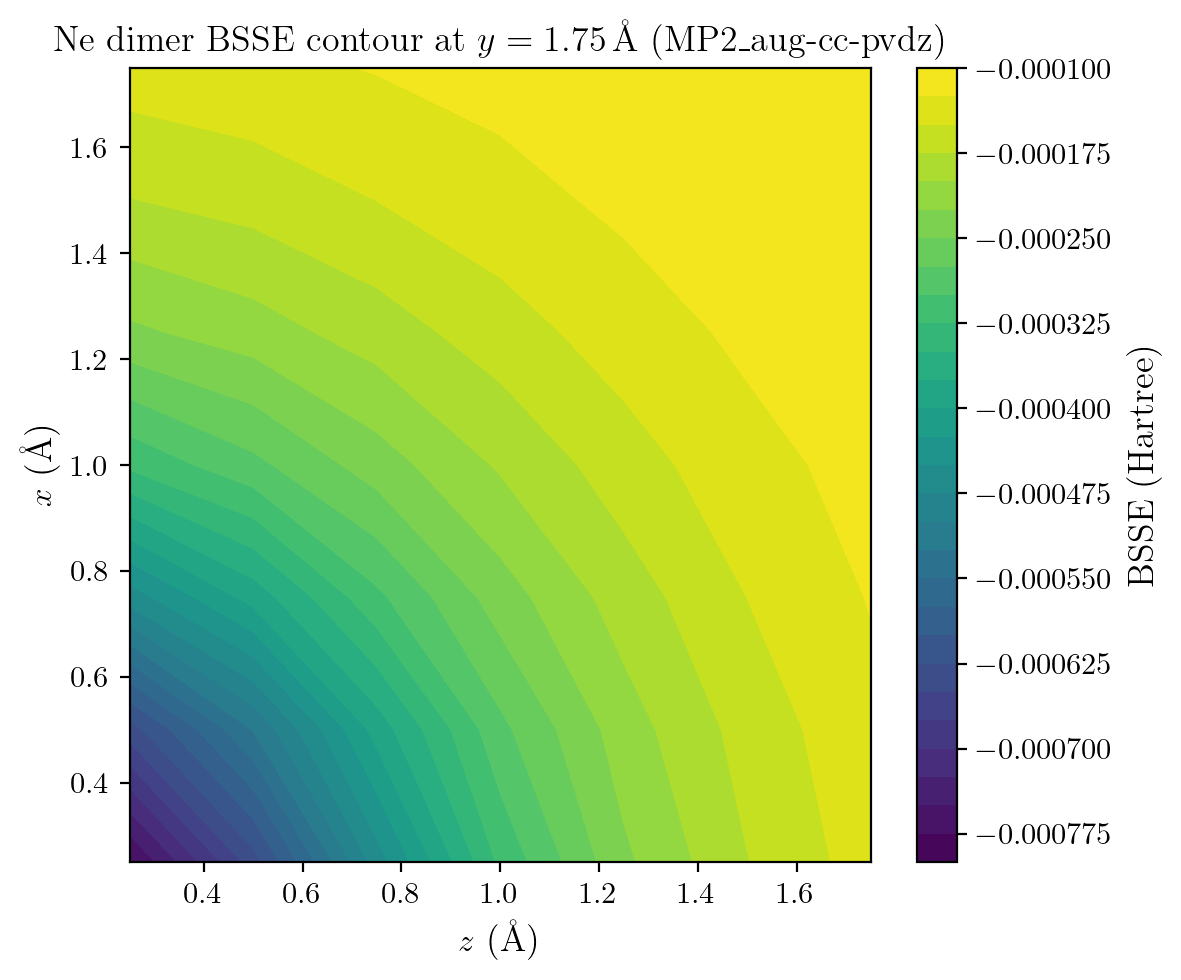
\includegraphics[width=\textwidth]{figures/dimer/Ne_dimer/Ne_trnl_contour_1.75_MP2.png}
        \caption{MP2 corr., $y = \SI{1.75}{\angstrom}$}
    \end{subfigure}
    \hfill
    \begin{subfigure}[b]{0.32\textwidth}
        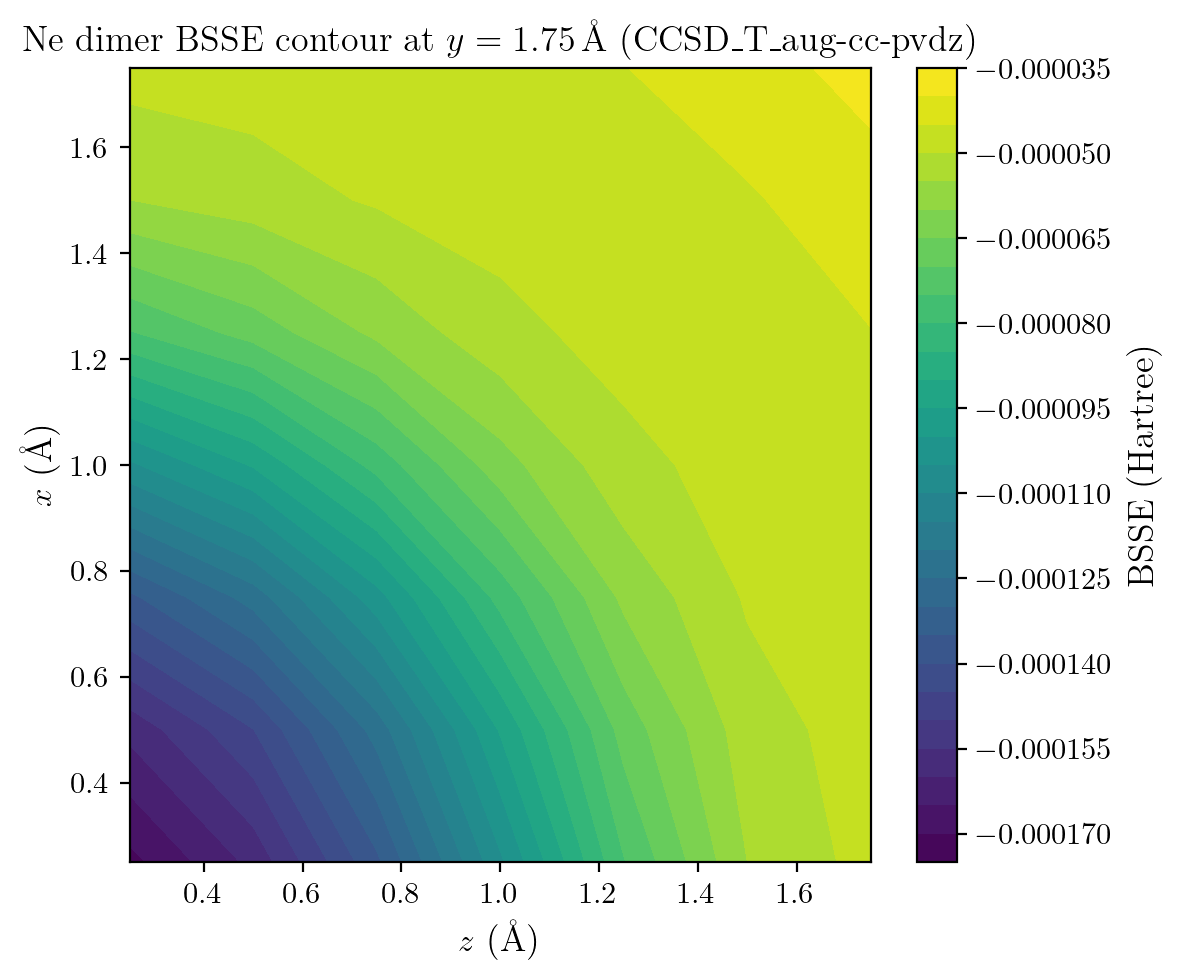
\includegraphics[width=\textwidth]{figures/dimer/Ne_dimer/Ne_trnl_contour_1.75_CCSD_T.png}
        \caption{CCSD(T) corr., $y = \SI{1.75}{\angstrom}$}
    \end{subfigure}

    \caption{BSSE contour plots for the Ne dimer translational scan at
    fixed $y = 1.5$ and \SI{1.75}{\angstrom}. Axes correspond to the
    in-plane Ne--Ne displacement components $(x, z)$ in \AA. Contour
    levels represent the BSSE in Hartree. The MP2 and CCSD(T) labels
    refer to the correlation energy components relative to SCF and MP2,
    respectively. The perfectly circular contour arcs confirm that BSSE
    depends only on the Ne--Ne separation $R$, with no orientational
    dependence, consistent with the spherical symmetry of the Ne atom.}
    \label{fig:ne_trnl_contours}
\end{figure}

The contour plots show perfectly circular arcs centered on the origin
at both $y$ values and across all three levels of theory. This confirms
that BSSE in the Ne dimer is a function only of the Ne--Ne distance
$R = |\mathbf{r}|$, with no dependence on the direction of the
displacement vector. The result is physically expected from the
spherical symmetry of Ne and serves as an important validation of the
computational setup.

Comparing the three methods, the MP2 correlation component shows the
largest BSSE magnitude, while the CCSD(T) increment beyond MP2 is
small. This ordering --- SCF $<$ CCSD(T) corr.\ $\ll$ MP2 corr.\ ---
is consistent across both $y$ slices and is characteristic of
correlated wavefunction methods applied to diffuse basis sets.

% ----------------------------------------------------------------------
\subsection{Key Findings}
% ----------------------------------------------------------------------

\begin{finding_box}
\textbf{Ne dimer BSSE is purely radial.}
The translational contour plots show perfectly circular arcs at both
sampled $y$ values and across all three levels of theory. BSSE in the
Ne dimer depends exclusively on the Ne--Ne separation $R$ with no
orientational dependence, as expected from the spherical symmetry of
the Ne atom. This result establishes a clean radial baseline against
which the orientational behavior of the polyatomic dimers (\ce{H2O}
and HF) can be compared.
\end{finding_box}

\begin{finding_box}
\textbf{MP2 correlation dominates the Ne dimer BSSE.}
Decomposing the total BSSE into SCF, MP2 correlation, and CCSD(T)
correlation components reveals that the MP2 contribution is the
largest at all sampled geometries. The CCSD(T) increment beyond MP2
is small. This energy decomposition hierarchy is consistent across
both $y$ slices and will be seen again in the \ce{H2O} and HF dimers.
\end{finding_box}

\clearpage

% ======================================================================
\section{\ce{H2O} Dimer}
% ======================================================================

% ----------------------------------------------------------------------
\subsection{Overview}
% ----------------------------------------------------------------------

The \ce{H2O} dimer serves as the central polyatomic case for this
study. Two complementary sampling strategies were employed to
characterize how BSSE depends on the relative geometry of the two
monomers: a \textit{translational scan}, in which monomer B is
displaced along a three-dimensional grid while monomer A remains
fixed, and a \textit{rotational--radial scan}, in which the Euler
angles $(\alpha, \beta, \gamma)$ of monomer B are sampled randomly
while the O--O separation $R$ is varied independently. All
calculations were performed at the SCF, MP2, and CCSD(T) levels using
the aug-cc-pVDZ basis set~\cite{dunning1989,kendall1992} with the
NWChem quantum chemistry package~\cite{nwchem2020}.

The BSSE for each dimer configuration is computed as in
Eq.~\eqref{eq:ne_dimer_bsse}, with $A$ and $B$ now denoting the two
\ce{H2O} monomers. Energies are reported in Hartree and distances
in \AA.

% ----------------------------------------------------------------------
\subsection{Experimental Design}
% ----------------------------------------------------------------------

\subsubsection{Monomer Geometry}

Both monomers use a rigid \ce{H2O} geometry. Monomer A is placed at
the origin with its oxygen atom and two hydrogen atoms fixed in the
$xy$ plane for all calculations. All coordinates are given in \AA,
consistent with the NWChem default convention.

\subsubsection{Translational Scan}

In the translational scan, the O--O displacement vector
$\mathbf{r} = \mathbf{r}_2 - \mathbf{r}_1$ (from the oxygen of
monomer A to the oxygen of monomer B) is varied in increments of
\SI{0.25}{\angstrom}. The scan is organized into three families of
two-dimensional slices:
\begin{itemize}
    \item Fixed $x$: contour over $(y, z)$
    \item Fixed $y$: contour over $(x, z)$
    \item Fixed $z$: contour over $(x, y)$
\end{itemize}
Only the fixed-$y$ slices at $y = 2.0$, $2.25$, $2.50$, and
\SI{2.75}{\angstrom} form complete $7 \times 7$ grids (49 points each)
and are used for contour analysis. The fixed-$x$ and fixed-$z$
families have incomplete grids and are excluded from the contour plots.

\subsubsection{Rotational--Radial Scan}

In the rotational--radial scan, the Euler angles $(\alpha, \beta,
\gamma)$ of monomer B are sampled randomly, producing 64 unique
orientations. For each orientation, the O--O separation $R$ is varied
independently. A total of 288 data points per method were collected.
Of the 64 orientations, 32 have at least 5 distinct $R$ values and
are used for plotting BSSE vs $R$ curves.

% ----------------------------------------------------------------------
\subsection{Translational Scan Results}
% ----------------------------------------------------------------------

Figure~\ref{fig:h2o_trnl_contours} shows the BSSE contour plots for
the fixed-$y$ slices at $y = 2.50$ and \SI{2.75}{\angstrom} for all
three levels of theory. Each panel shows BSSE as a function of the
in-plane coordinates $(x, z)$.

\begin{figure}[!ht]
    \centering
    \begin{subfigure}[b]{0.32\textwidth}
        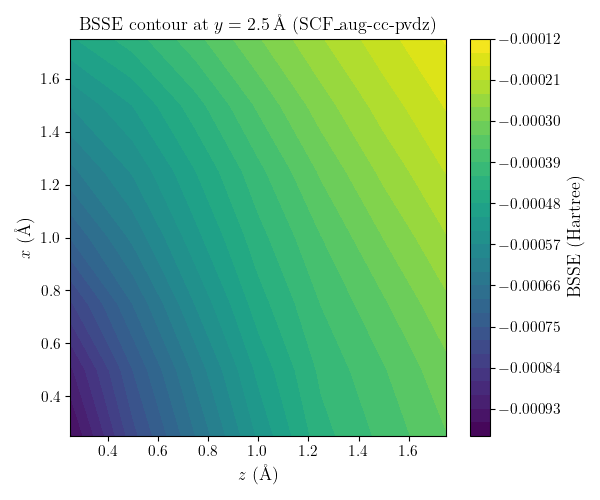
\includegraphics[width=\textwidth]{figures/dimer/H2O_dimer/H2O_trnl_contour_2.50_SCF.png}
        \caption{SCF, $y = \SI{2.50}{\angstrom}$}
    \end{subfigure}
    \hfill
    \begin{subfigure}[b]{0.32\textwidth}
        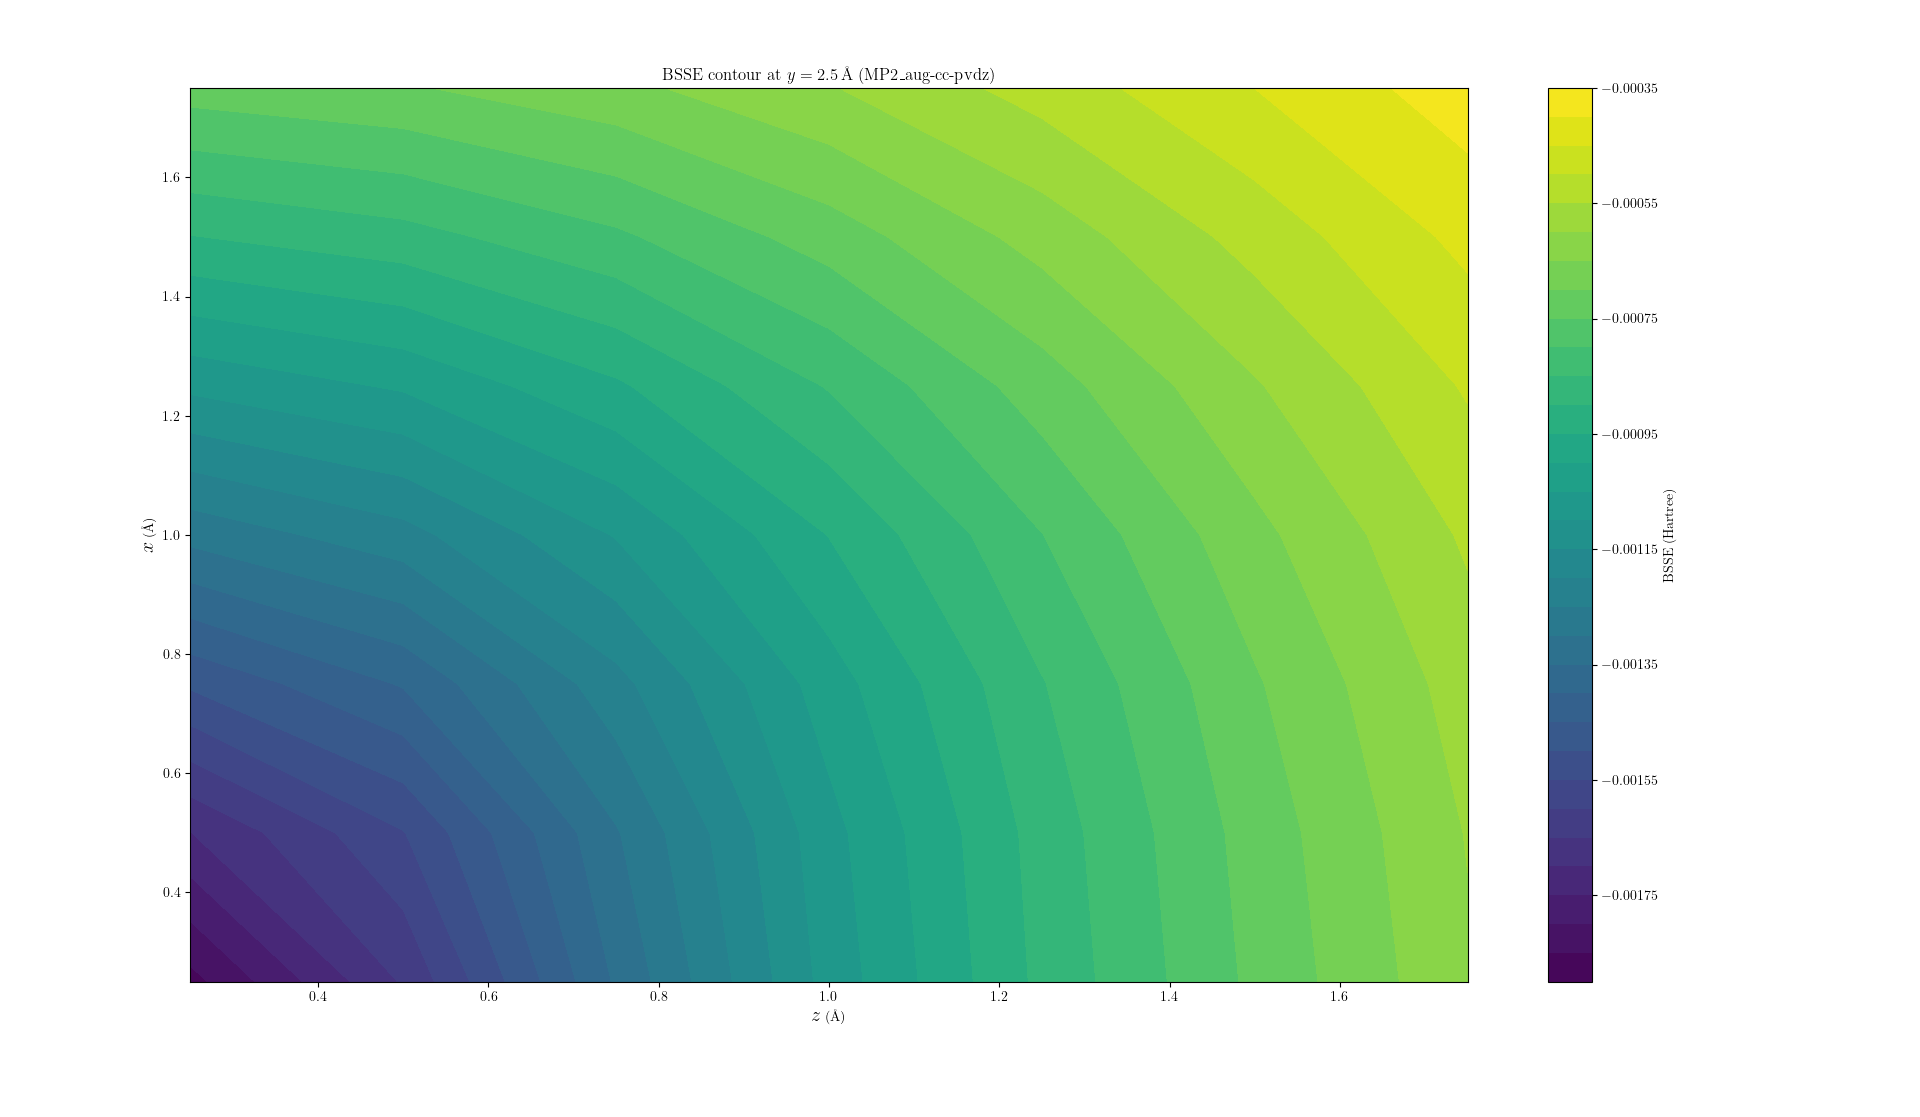
\includegraphics[width=\textwidth]{figures/dimer/H2O_dimer/H2O_trnl_contour_2.50_MP2.png}
        \caption{MP2 corr., $y = \SI{2.50}{\angstrom}$}
    \end{subfigure}
    \hfill
    \begin{subfigure}[b]{0.32\textwidth}
        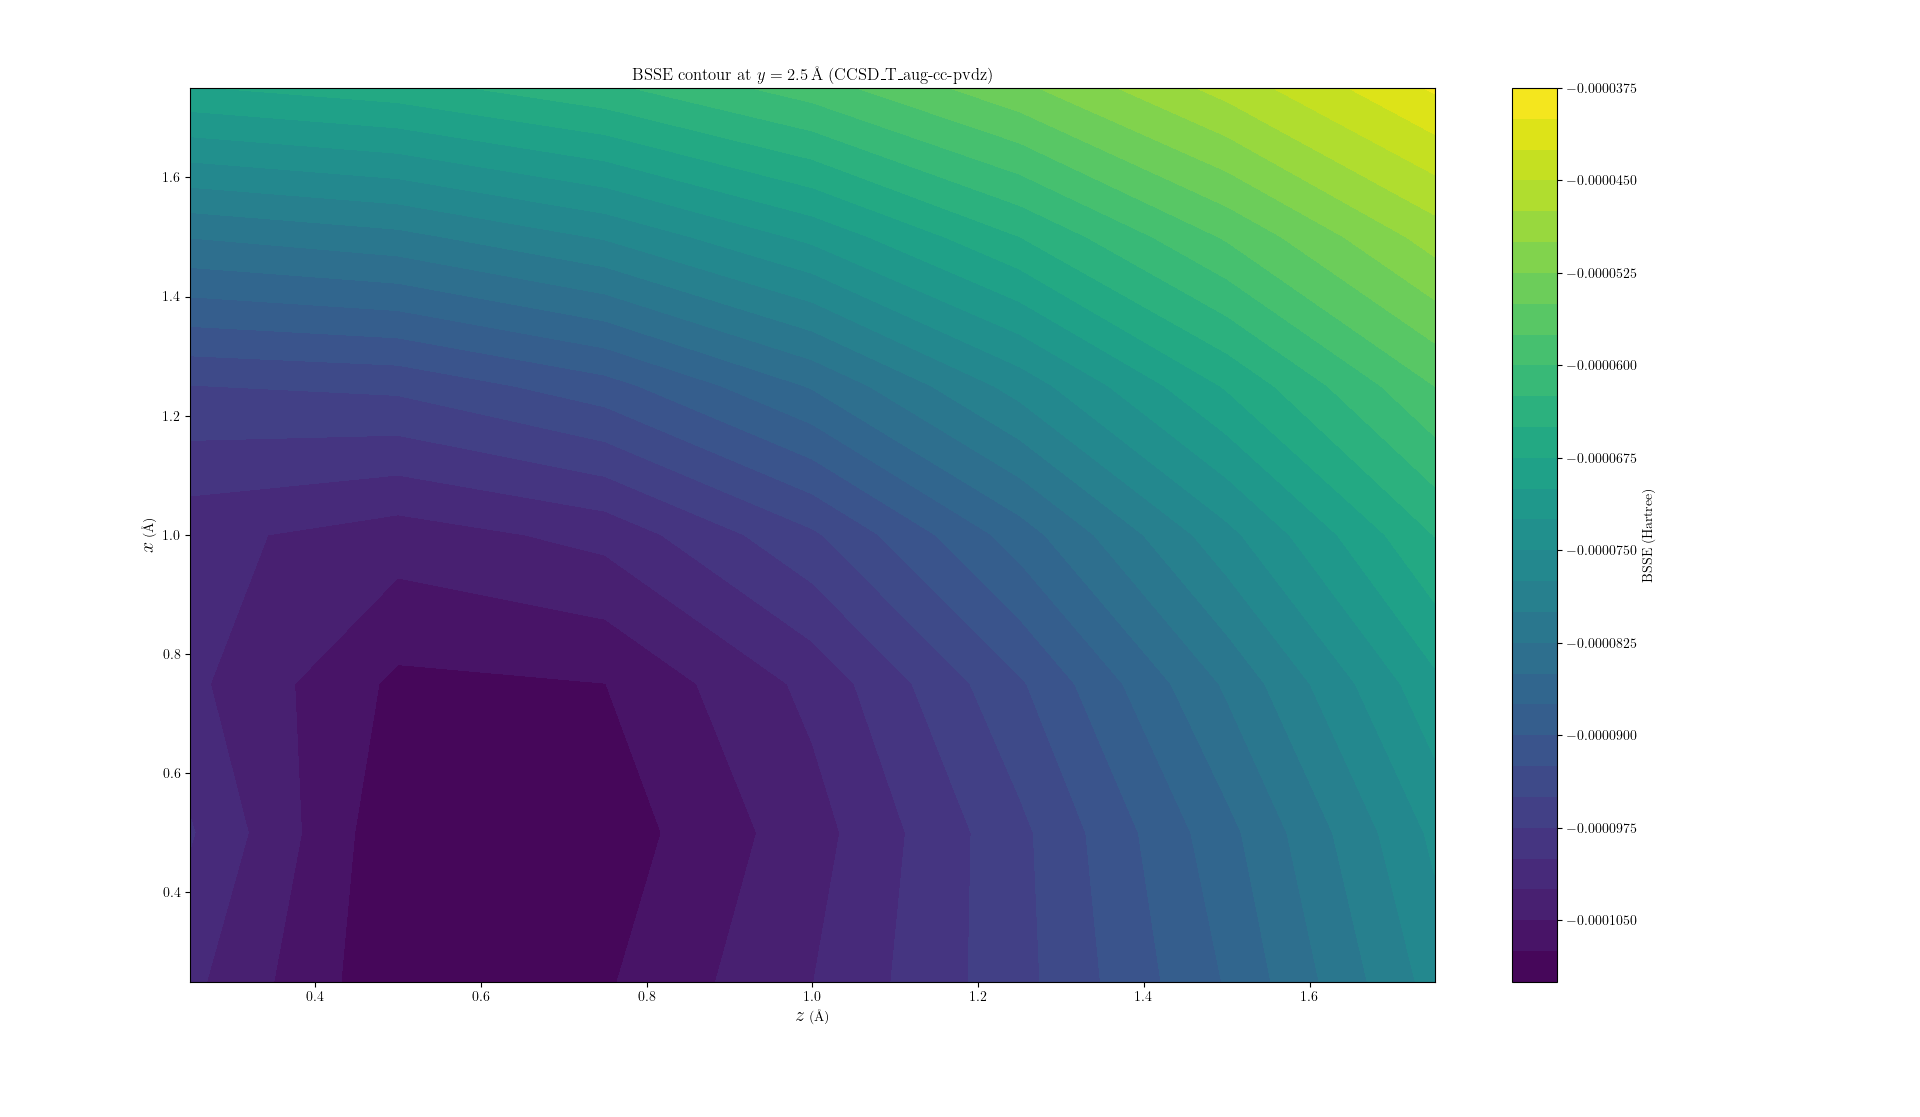
\includegraphics[width=\textwidth]{figures/dimer/H2O_dimer/H2O_trnl_contour_2.50_CCSD_T.png}
        \caption{CCSD(T) corr., $y = \SI{2.50}{\angstrom}$}
    \end{subfigure}

    \vspace{0.8em}

    \begin{subfigure}[b]{0.32\textwidth}
        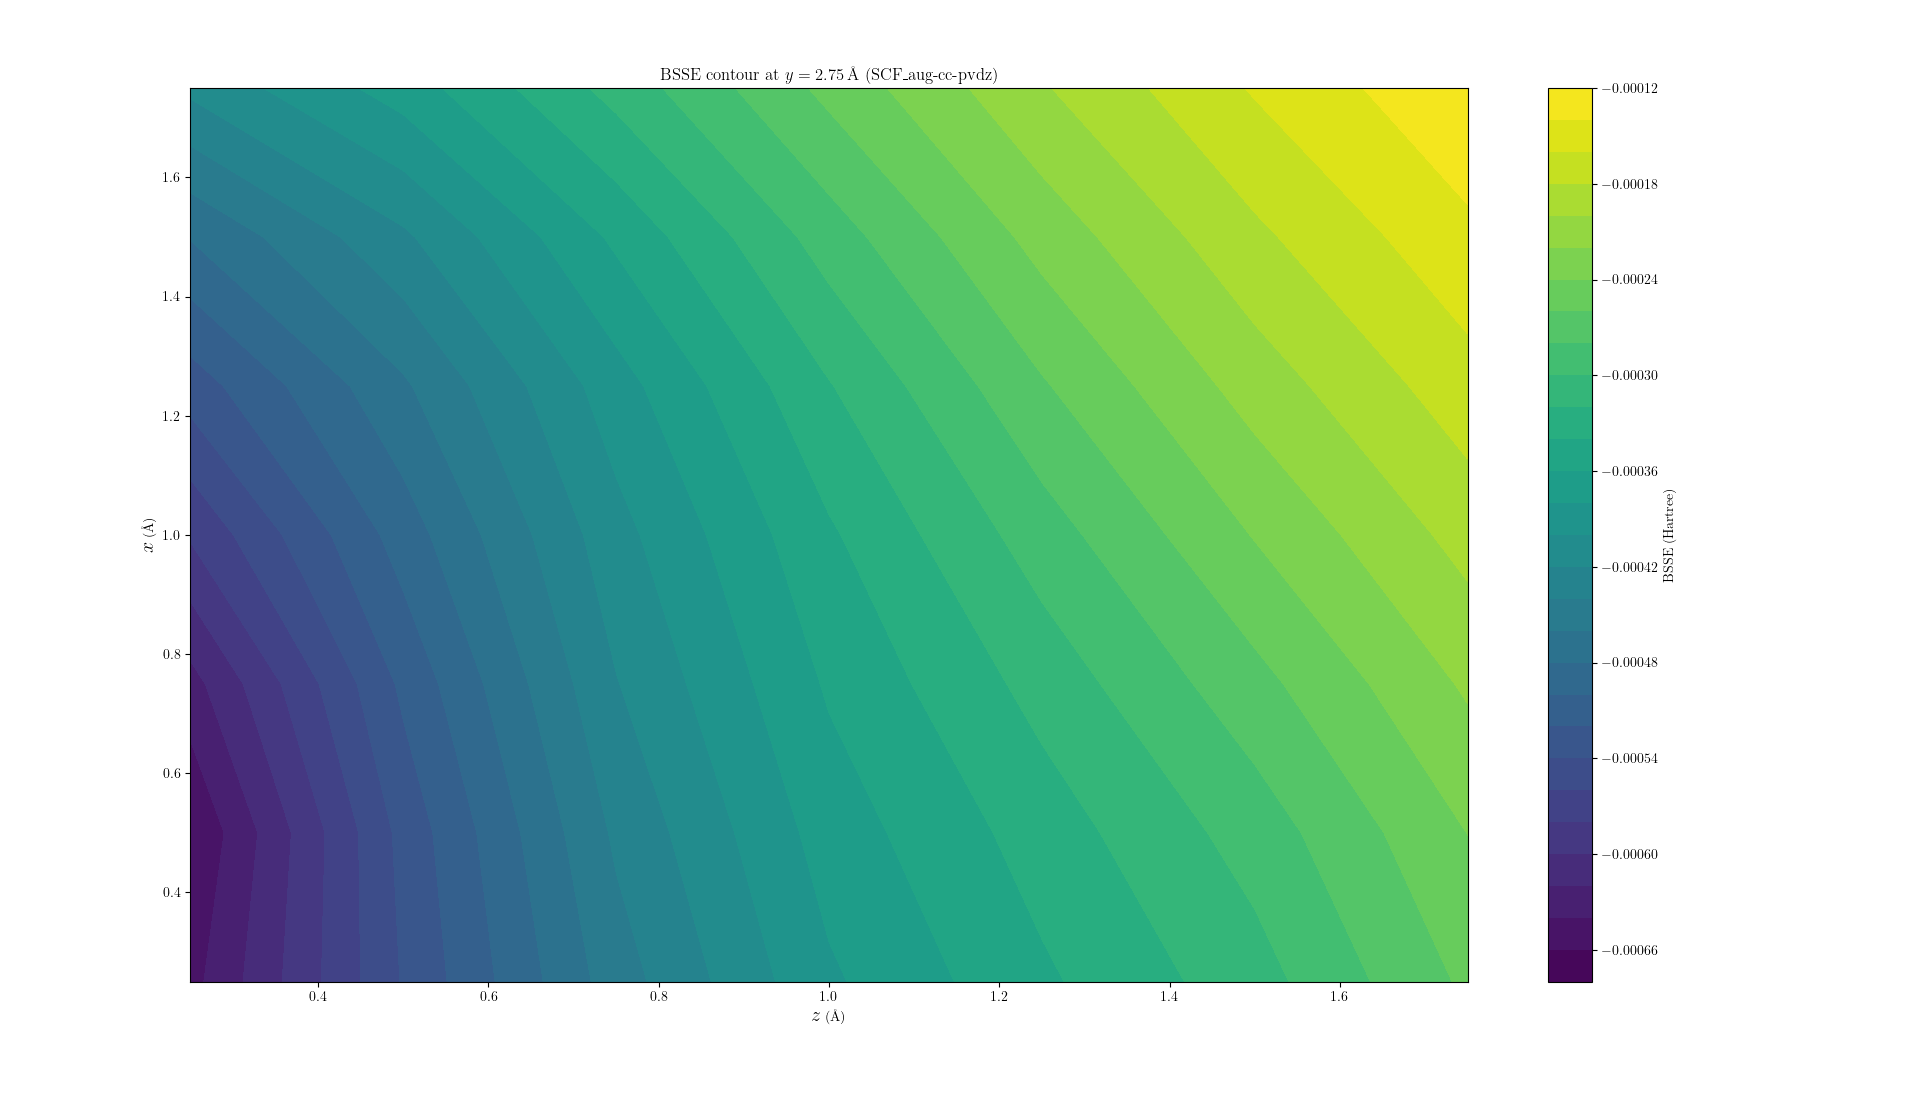
\includegraphics[width=\textwidth]{figures/dimer/H2O_dimer/H2O_trnl_contour_2.75_SCF.png}
        \caption{SCF, $y = \SI{2.75}{\angstrom}$}
    \end{subfigure}
    \hfill
    \begin{subfigure}[b]{0.32\textwidth}
        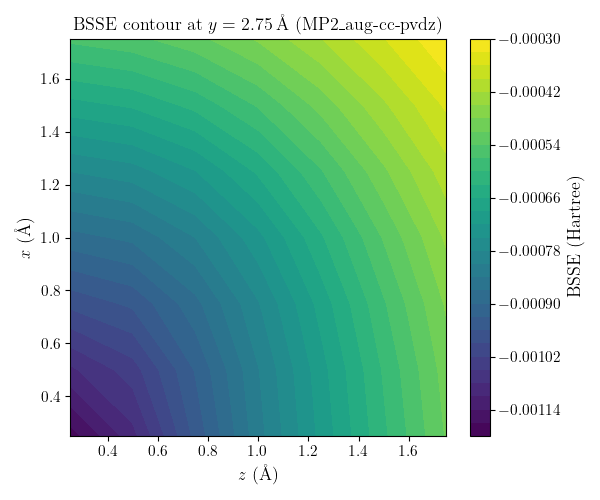
\includegraphics[width=\textwidth]{figures/dimer/H2O_dimer/H2O_trnl_contour_2.75_MP2.png}
        \caption{MP2 corr., $y = \SI{2.75}{\angstrom}$}
    \end{subfigure}
    \hfill
    \begin{subfigure}[b]{0.32\textwidth}
        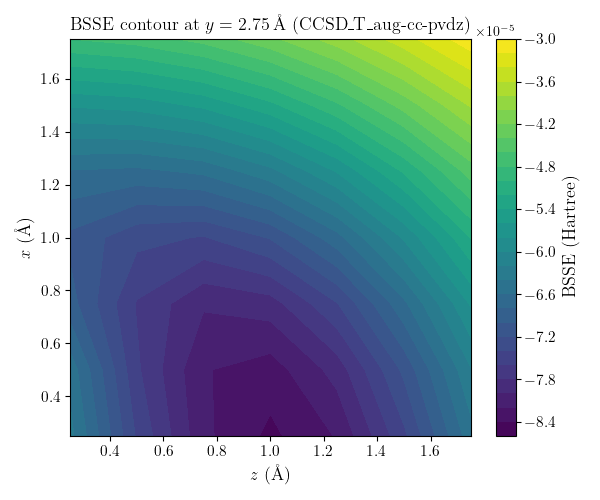
\includegraphics[width=\textwidth]{figures/dimer/H2O_dimer/H2O_trnl_contour_2.75_CCSD_T.png}
        \caption{CCSD(T) corr., $y = \SI{2.75}{\angstrom}$}
    \end{subfigure}

    \caption{BSSE contour plots for the \ce{H2O} dimer translational
    scan at fixed $y = 2.50$ and \SI{2.75}{\angstrom}. Axes correspond
    to the in-plane O--O displacement components $(x, z)$ in \AA.
    Contour levels represent the BSSE in Hartree. The MP2 and CCSD(T)
    labels refer to the correlation energy components relative to SCF
    and MP2, respectively. The nearly circular contour arcs indicate
    that BSSE depends primarily on the O--O separation $R$ with weak
    orientation dependence.}
    \label{fig:h2o_trnl_contours}
\end{figure}

The contour plots reveal nearly circular arcs centered on the origin,
indicating that BSSE is predominantly a function of the O--O distance
$R = |\mathbf{r}|$ with only weak dependence on the direction of the
displacement vector. This observation holds across all three levels of
theory and all four fixed-$y$ slices. In contrast to the Ne dimer,
the contours are not perfectly circular --- a small but visible
deviation from circular symmetry reflects the non-spherical geometry
of the \ce{H2O} monomer.

% ----------------------------------------------------------------------
\subsection{Rotational--Radial Scan Results}
% ----------------------------------------------------------------------

Figure~\ref{fig:h2o_rot_bsse_vs_R} shows $|\text{BSSE}|$ as a
function of $R$ for 9 representative orientations, with SCF, MP2
correlation, and CCSD(T) correlation components overlaid on each
panel.

Several observations are consistent across all 9 orientations:

\begin{enumerate}
    \item \textbf{Monotonic decay with $R$.} All three components
    decrease monotonically as the O--O separation increases,
    approaching zero at large $R$.

    \item \textbf{Dominance of the MP2 correlation component.} The
    MP2 correlation contribution to BSSE is the largest of the three
    components across all orientations and distances sampled.
    % At the
    % SCF level, only the occupied molecular orbitals contribute to the
    % electron density, and the basis set incompleteness error arises
    % from the inability of the monomer's own basis to describe these
    % occupied orbitals in the field of the partner. At the MP2 level,
    % the correlation energy is computed through excitations into virtual
    % orbitals, which are typically more diffuse and more sensitive to
    % basis set incompleteness than the occupied orbitals. As a result,
    % the correlated wavefunction benefits more from borrowing the
    % partner's basis functions --- the ghost atoms effectively provide
    % additional virtual space that the monomer's own basis lacks. This
    % amplification of BSSE by electron correlation is a well-known
    % phenomenon and is one of the primary motivations for using
    % augmented basis sets such as aug-cc-pVDZ in BSSE studies.

    \item \textbf{Small CCSD(T) increment.} The CCSD(T) correlation
    component is consistently small relative to both SCF and MP2
    contributions.
    % suggesting that higher-order correlation effects
    % beyond MP2 contribute minimally to the BSSE.

    \item \textbf{Weak orientation dependence.} The shape and
    magnitude of the BSSE curves are consistent across different
    $(\alpha, \beta, \gamma)$ values, in agreement with the nearly
    circular contour arcs observed in the translational scan.
\end{enumerate}

\vspace{0.25cm}
\begin{figure}[!ht]
    \centering
    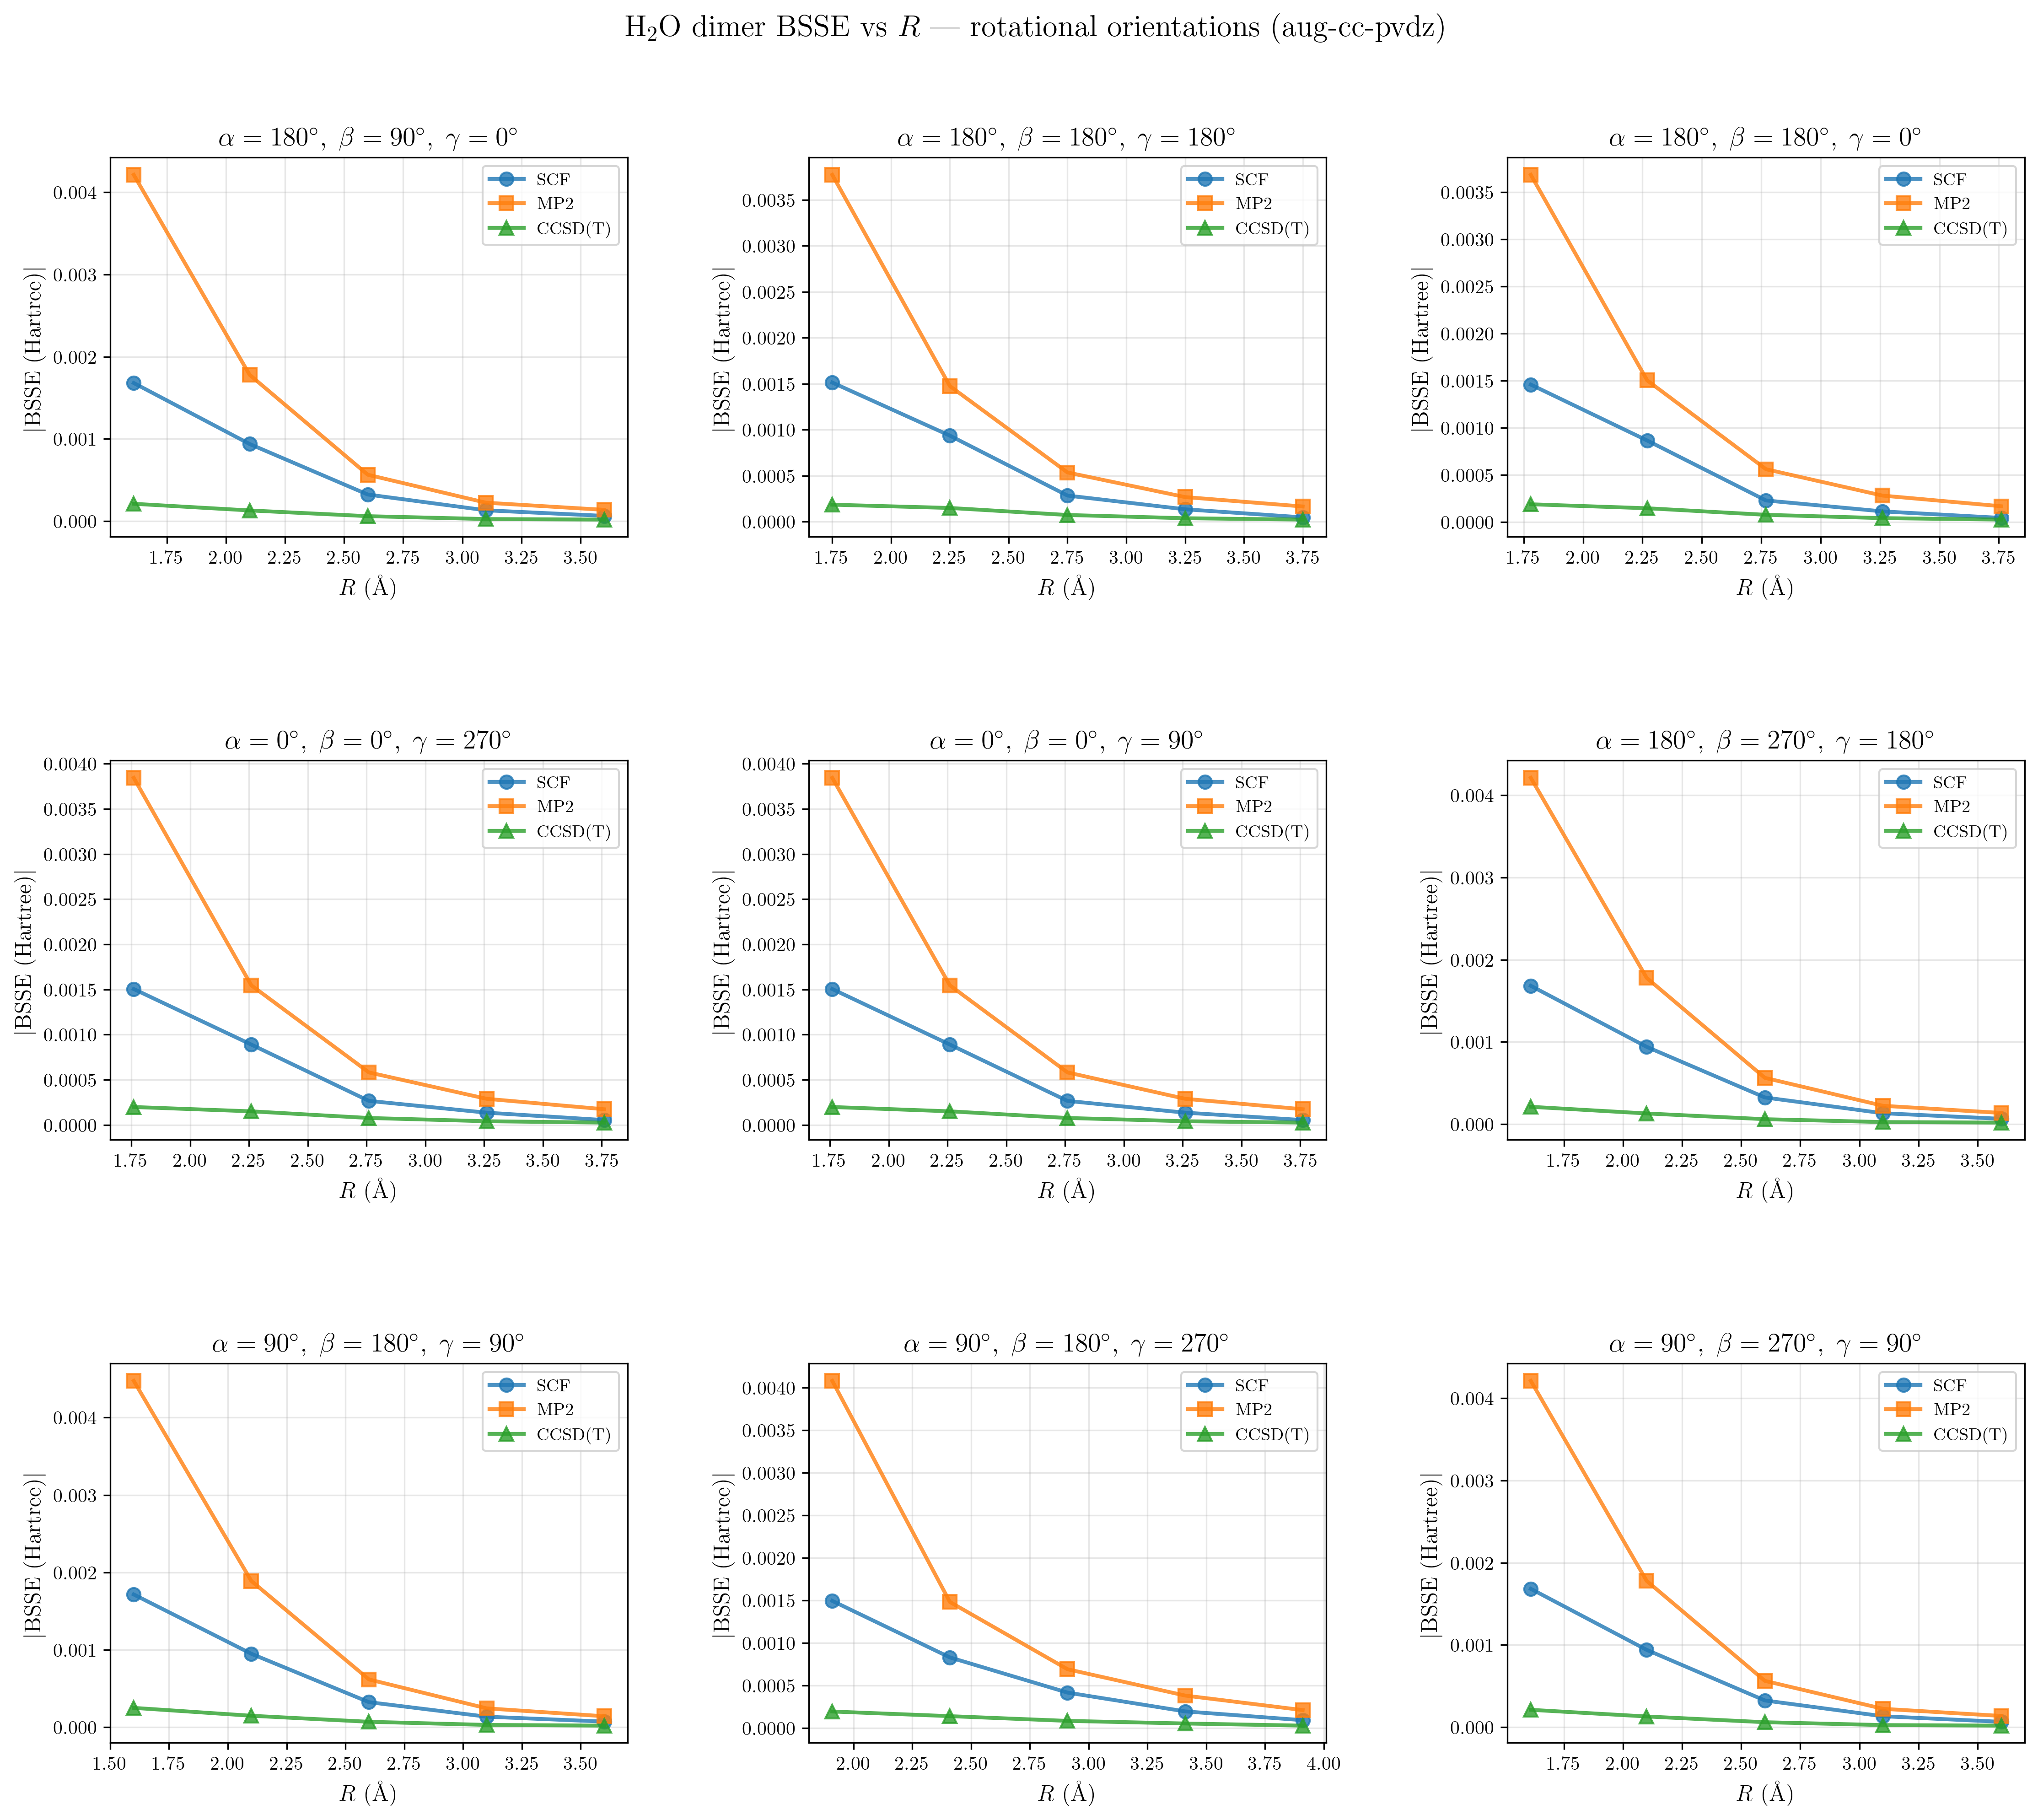
\includegraphics[width=1.0\textwidth]{figures/dimer/H2O_dimer/H2O_rot_vs_R_SCFMP2CCSD_T.png}
    \caption{$|\text{BSSE}|$ vs O--O separation $R$ for 9
    representative rotational orientations of the \ce{H2O} dimer at
    the aug-cc-pVDZ level. Each panel corresponds to a distinct set of
    Euler angles $(\alpha, \beta, \gamma)$ as labeled. Blue circles:
    SCF contribution; orange squares: MP2 correlation component
    ($E_\text{MP2} - E_\text{SCF}$); green triangles: CCSD(T)
    correlation component ($E_{\text{CCSD(T)}} - E_\text{MP2}$).
    All three components decay monotonically with $R$ and show
    consistent behavior across orientations, confirming weak
    orientation dependence of dimer BSSE.}
    \label{fig:h2o_rot_bsse_vs_R}
\end{figure}

\clearpage

% ----------------------------------------------------------------------
\subsection{Key Findings}
% ----------------------------------------------------------------------

\begin{finding_box}
\textbf{\ce{H2O} dimer BSSE is primarily a function of O--O distance.}
Both the translational contour plots and the rotational--radial scan
confirm that BSSE in the \ce{H2O} dimer depends weakly on the relative
orientation of the monomers and is governed primarily by the O--O
separation $R$. The nearly circular contour arcs represent a modest
deviation from the perfect circular symmetry seen in the Ne dimer,
consistent with the non-spherical geometry of the \ce{H2O} monomer.
% This result motivates the hypothesis that a simple
% distance-based threshold could be used to identify configurations
% where BSSE corrections are negligible.
\end{finding_box}

\begin{finding_box}
\textbf{MP2 correlation dominates the \ce{H2O} dimer BSSE.}
Decomposing the total BSSE into SCF, MP2 correlation, and CCSD(T)
correlation components reveals that the MP2 contribution is the
largest at all sampled distances and orientations. The CCSD(T)
correction beyond MP2 is small.
% This energy decomposition hierarchy
% provides essential context for the trimer analysis presented in
% Chapters~\ref{ch:trimer_bsse} and~\ref{ch:trimer_interaction}.
\end{finding_box}

\clearpage

% ======================================================================
\section{HF Dimer}
% ======================================================================

% ----------------------------------------------------------------------
\subsection{Overview}
% ----------------------------------------------------------------------

The HF dimer completes the set of three dimer systems studied in this
work. As a polar, heteronuclear diatomic, HF introduces a qualitative
distinction from both Ne and \ce{H2O}: the two ends of the molecule
are chemically inequivalent, so the direction of the displacement
vector relative to the HF bond axis can in principle affect the BSSE.
Two complementary sampling strategies were employed, mirroring the
\ce{H2O} analysis: a \textit{translational scan}, in which monomer B
is displaced along a three-dimensional grid while monomer A remains
fixed, and a \textit{rotational--radial scan}, in which the Euler
angles $(\alpha, \beta, \gamma)$ of monomer B are varied
systematically while the F--F separation $R$ is held fixed. All
calculations were performed at the SCF, MP2, and CCSD(T) levels using
the aug-cc-pVDZ basis set~\cite{dunning1989,kendall1992} with the
NWChem quantum chemistry package~\cite{nwchem2020}.

The BSSE for each dimer configuration is computed as in
Eq.~\eqref{eq:ne_dimer_bsse}, with $A$ and $B$ now denoting the two
HF monomers. Energies are reported in Hartree and distances in \AA.

% ----------------------------------------------------------------------
\subsection{Experimental Design}
% ----------------------------------------------------------------------

\subsubsection{Monomer Geometry}

Monomer A is placed at the origin with the HF bond axis fixed in the
$xy$ plane for all calculations. The HF bond length is approximately
\SI{0.924}{\angstrom}. All coordinates are given in \AA, consistent
with the NWChem default convention.

\subsubsection{Translational Scan}

The translational scan follows the same protocol as the \ce{H2O}
dimer. The F--F displacement vector $\mathbf{r} = \mathbf{r}_2 -
\mathbf{r}_1$ is varied in increments of \SI{0.25}{\angstrom}. Only
the fixed-$y$ slices at $y = 1.5$ and $y = \SI{1.75}{\angstrom}$
form complete $7 \times 7$ grids (49 points each) and are used for
contour analysis. The axes of each contour plot correspond to the
in-plane F--F displacement components $(x, z)$ in \AA.

\subsubsection{Rotational--Radial Scan}

In the rotational--radial scan, the Euler angles of monomer B are
varied systematically rather than randomly. A total of 152
orientations were generated, all with $\alpha = 90.0°$. Of these, 28
have at least 5 distinct $R$ values and are used for plotting BSSE
vs $R$ curves. This systematic sampling contrasts with the random
Euler angle sampling used for \ce{H2O} and provides denser coverage
of a specific rotational subspace.

% ----------------------------------------------------------------------
\subsection{Translational Scan Results}
% ----------------------------------------------------------------------

Figure~\ref{fig:hf_trnl_contours} shows the BSSE contour plots for
the fixed-$y$ slices at $y = 1.5$ and \SI{1.75}{\angstrom} for all
three levels of theory.

\begin{figure}[!ht]
    \centering
    \begin{subfigure}[b]{0.32\textwidth}
        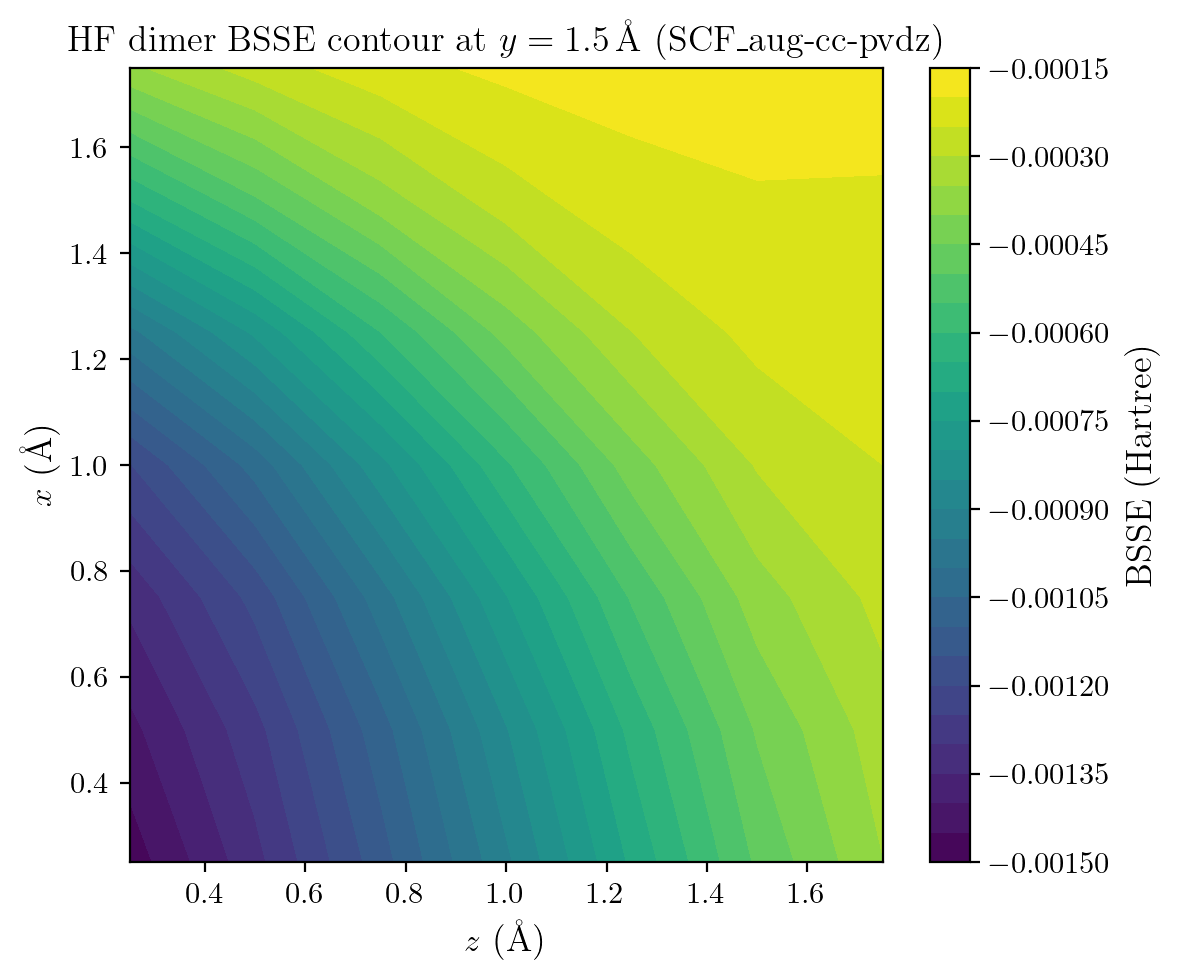
\includegraphics[width=\textwidth]{figures/dimer/HF_dimer/HF_trnl_contour_1.5_SCF.png}
        \caption{SCF, $y = \SI{1.5}{\angstrom}$}
    \end{subfigure}
    \hfill
    \begin{subfigure}[b]{0.32\textwidth}
        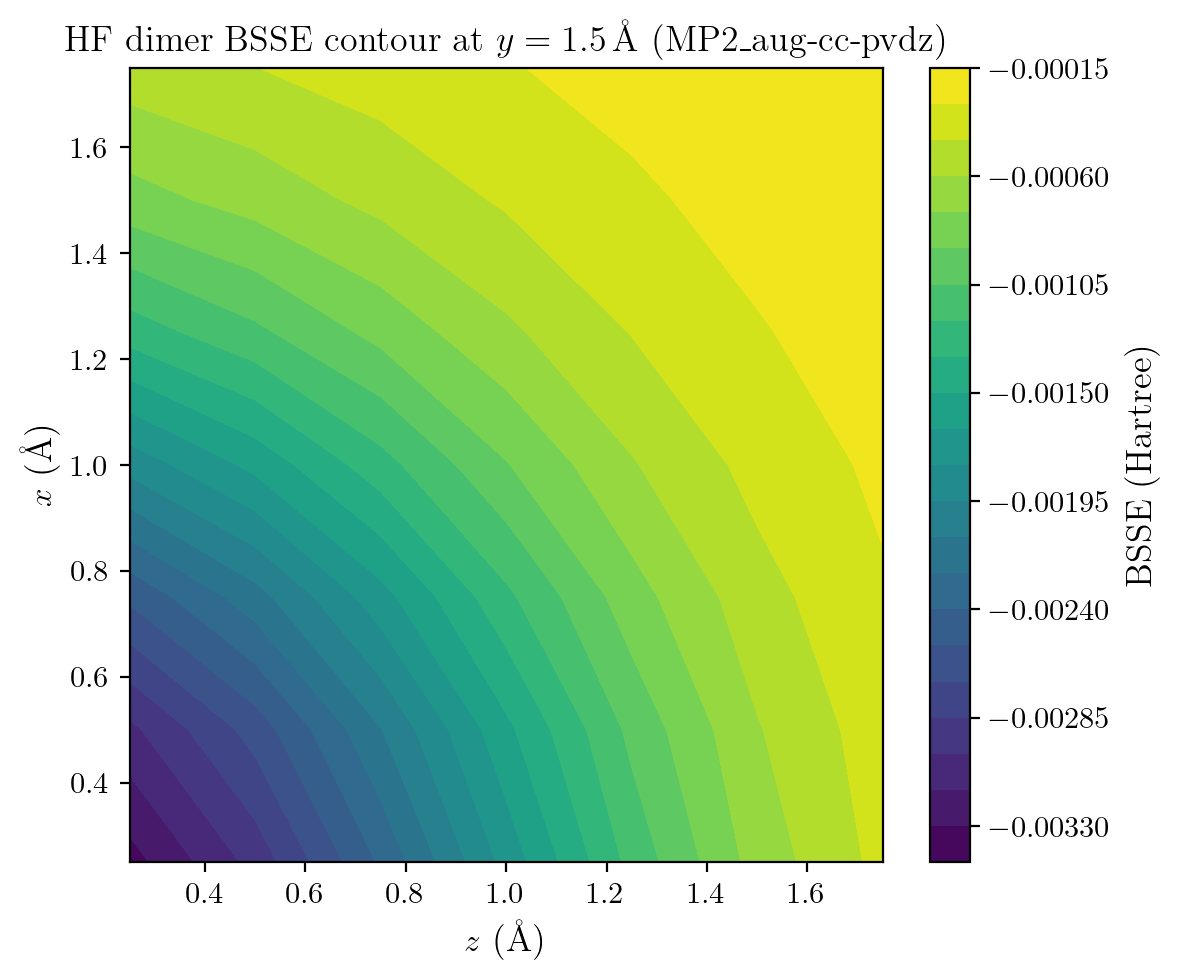
\includegraphics[width=\textwidth]{figures/dimer/HF_dimer/HF_trnl_contour_1.5_MP2.png}
        \caption{MP2 corr., $y = \SI{1.5}{\angstrom}$}
    \end{subfigure}
    \hfill
    \begin{subfigure}[b]{0.32\textwidth}
        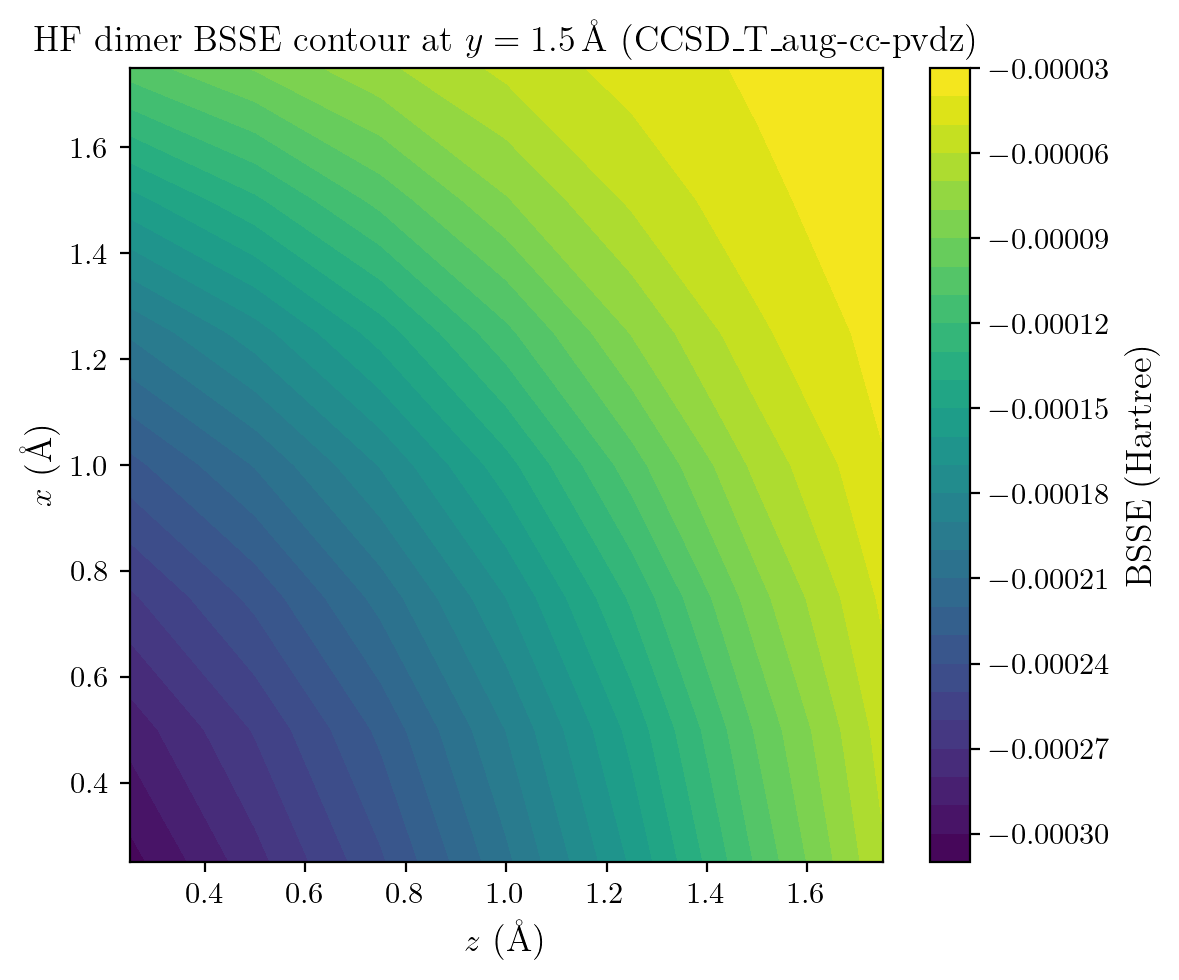
\includegraphics[width=\textwidth]{figures/dimer/HF_dimer/HF_trnl_contour_1.5_CCSD_T.png}
        \caption{CCSD(T) corr., $y = \SI{1.5}{\angstrom}$}
    \end{subfigure}

    \vspace{0.8em}

    \begin{subfigure}[b]{0.32\textwidth}
        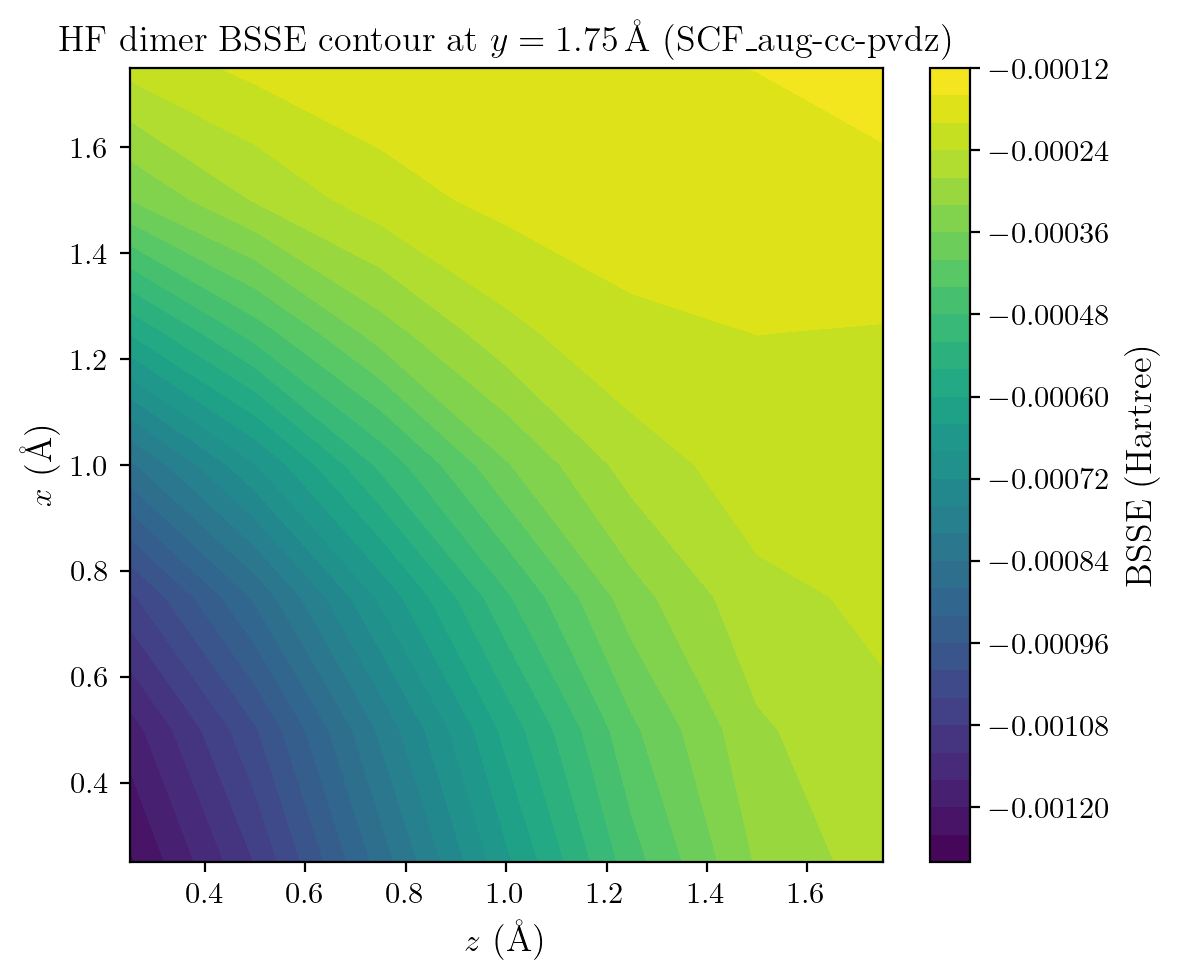
\includegraphics[width=\textwidth]{figures/dimer/HF_dimer/HF_trnl_contour_1.75_SCF.png}
        \caption{SCF, $y = \SI{1.75}{\angstrom}$}
    \end{subfigure}
    \hfill
    \begin{subfigure}[b]{0.32\textwidth}
        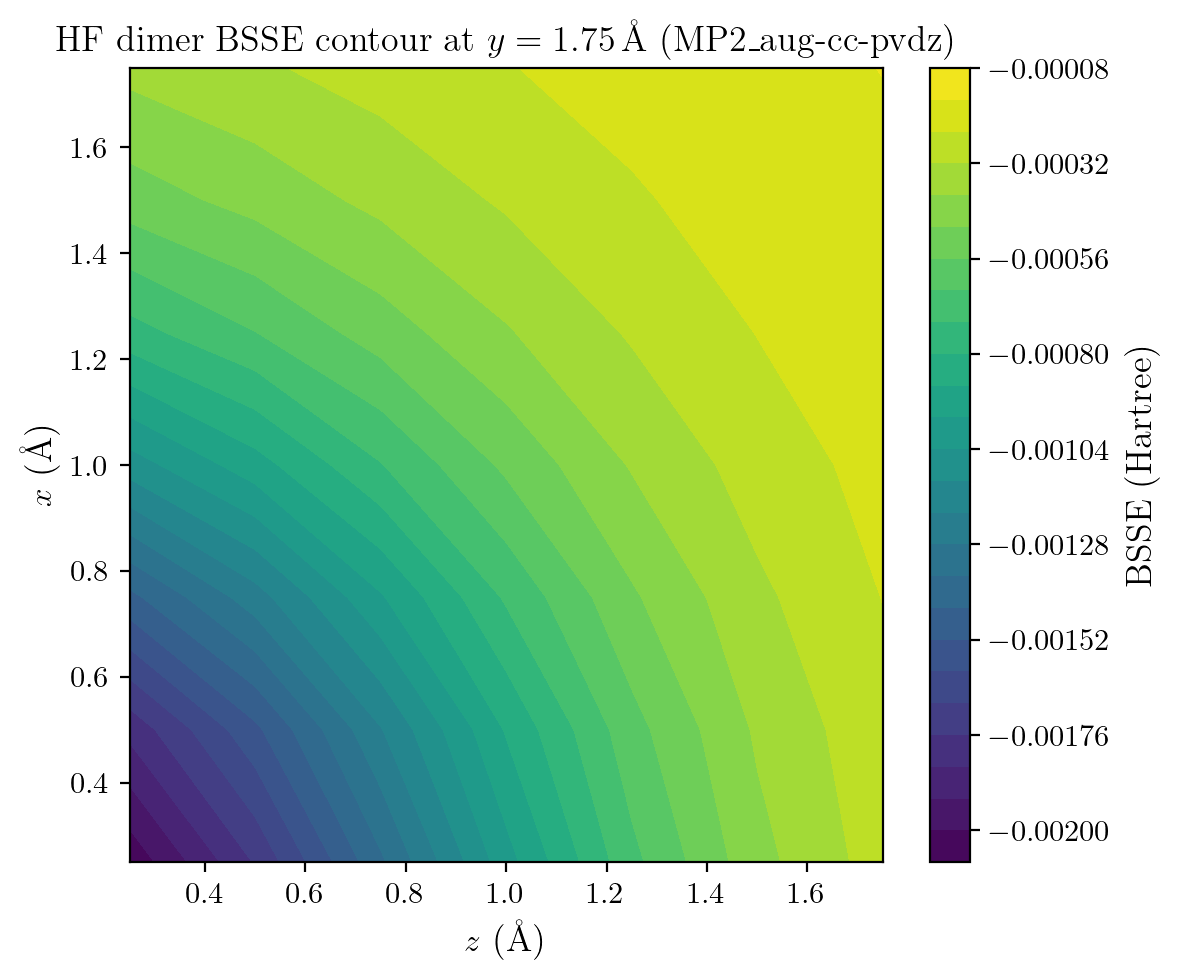
\includegraphics[width=\textwidth]{figures/dimer/HF_dimer/HF_trnl_contour_1.75_MP2.png}
        \caption{MP2 corr., $y = \SI{1.75}{\angstrom}$}
    \end{subfigure}
    \hfill
    \begin{subfigure}[b]{0.32\textwidth}
        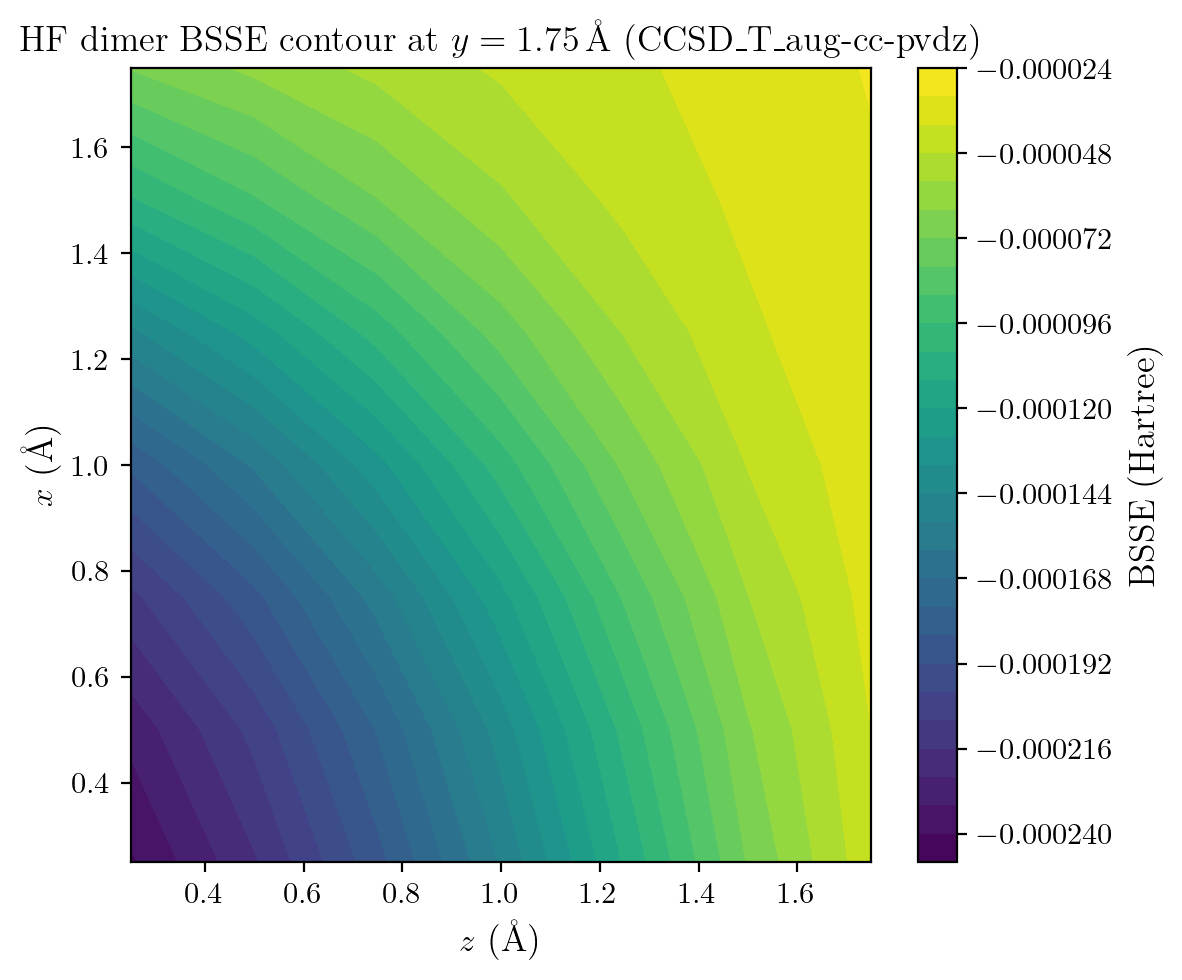
\includegraphics[width=\textwidth]{figures/dimer/HF_dimer/HF_trnl_contour_1.75_CCSD_T.png}
        \caption{CCSD(T) corr., $y = \SI{1.75}{\angstrom}$}
    \end{subfigure}

    \caption{BSSE contour plots for the HF dimer translational scan at
    fixed $y = 1.5$ and \SI{1.75}{\angstrom}. Axes correspond to the
    in-plane F--F displacement components $(x, z)$ in \AA. Contour
    levels represent the BSSE in Hartree. The MP2 and CCSD(T) labels
    refer to the correlation energy components relative to SCF and MP2,
    respectively. At $y = \SI{1.5}{\angstrom}$ all three methods show
    nearly circular contours; at $y = \SI{1.75}{\angstrom}$ the SCF
    contours develop a visible asymmetry between the $x$ and $z$
    directions, reflecting the polar and heteronuclear character of
    the HF monomer.}
    \label{fig:hf_trnl_contours}
\end{figure}

At $y = \SI{1.5}{\angstrom}$, all three methods show nearly circular
contour arcs, consistent with the behavior observed for Ne and
\ce{H2O}. At $y = \SI{1.75}{\angstrom}$, the MP2 and CCSD(T)
contours remain circular, but the SCF contours develop a visible
asymmetry between the $x$ and $z$ directions.

%----------------------------------------------------------------------
% TODO: pending PI discussion — physical interpretation of SCF asymmetry
%-----------------------------------------------------------------------
% This asymmetry is a physical effect, not a numerical artifact. The
% computational grid was verified to be perfectly symmetric (a $7 \times
% 7$ grid with identical $x$ and $z$ ranges), ruling out any grid
% artifact. The origin of the asymmetry lies in the heteronuclear nature
% of HF: unlike Ne (spherically symmetric) and \ce{H2O} (which has a
% $C_{2v}$ symmetry axis), HF has distinct H and F ends. At
% $y = \SI{1.75}{\angstrom}$ the in-plane displacement components become
% comparable to the HF bond length (\SI{0.924}{\angstrom}), making the
% orientation of H vs F relative to the displacement direction
% observable in the SCF BSSE. The fact that this asymmetry appears at
% the SCF level but not in the MP2 and CCSD(T) correlation components
% suggests it arises from the anisotropy of the SCF electron density of
% the HF monomer rather than from correlation effects.

\clearpage
% ----------------------------------------------------------------------
\subsection{Rotational--Radial Scan Results}
% ----------------------------------------------------------------------

Figure~\ref{fig:hf_rot_bsse_vs_R} shows $|\text{BSSE}|$ as a function
of $R$ for 9 representative orientations, with SCF, MP2 correlation,
and CCSD(T) correlation components overlaid on each panel.

\begin{figure}[H]
    \centering
    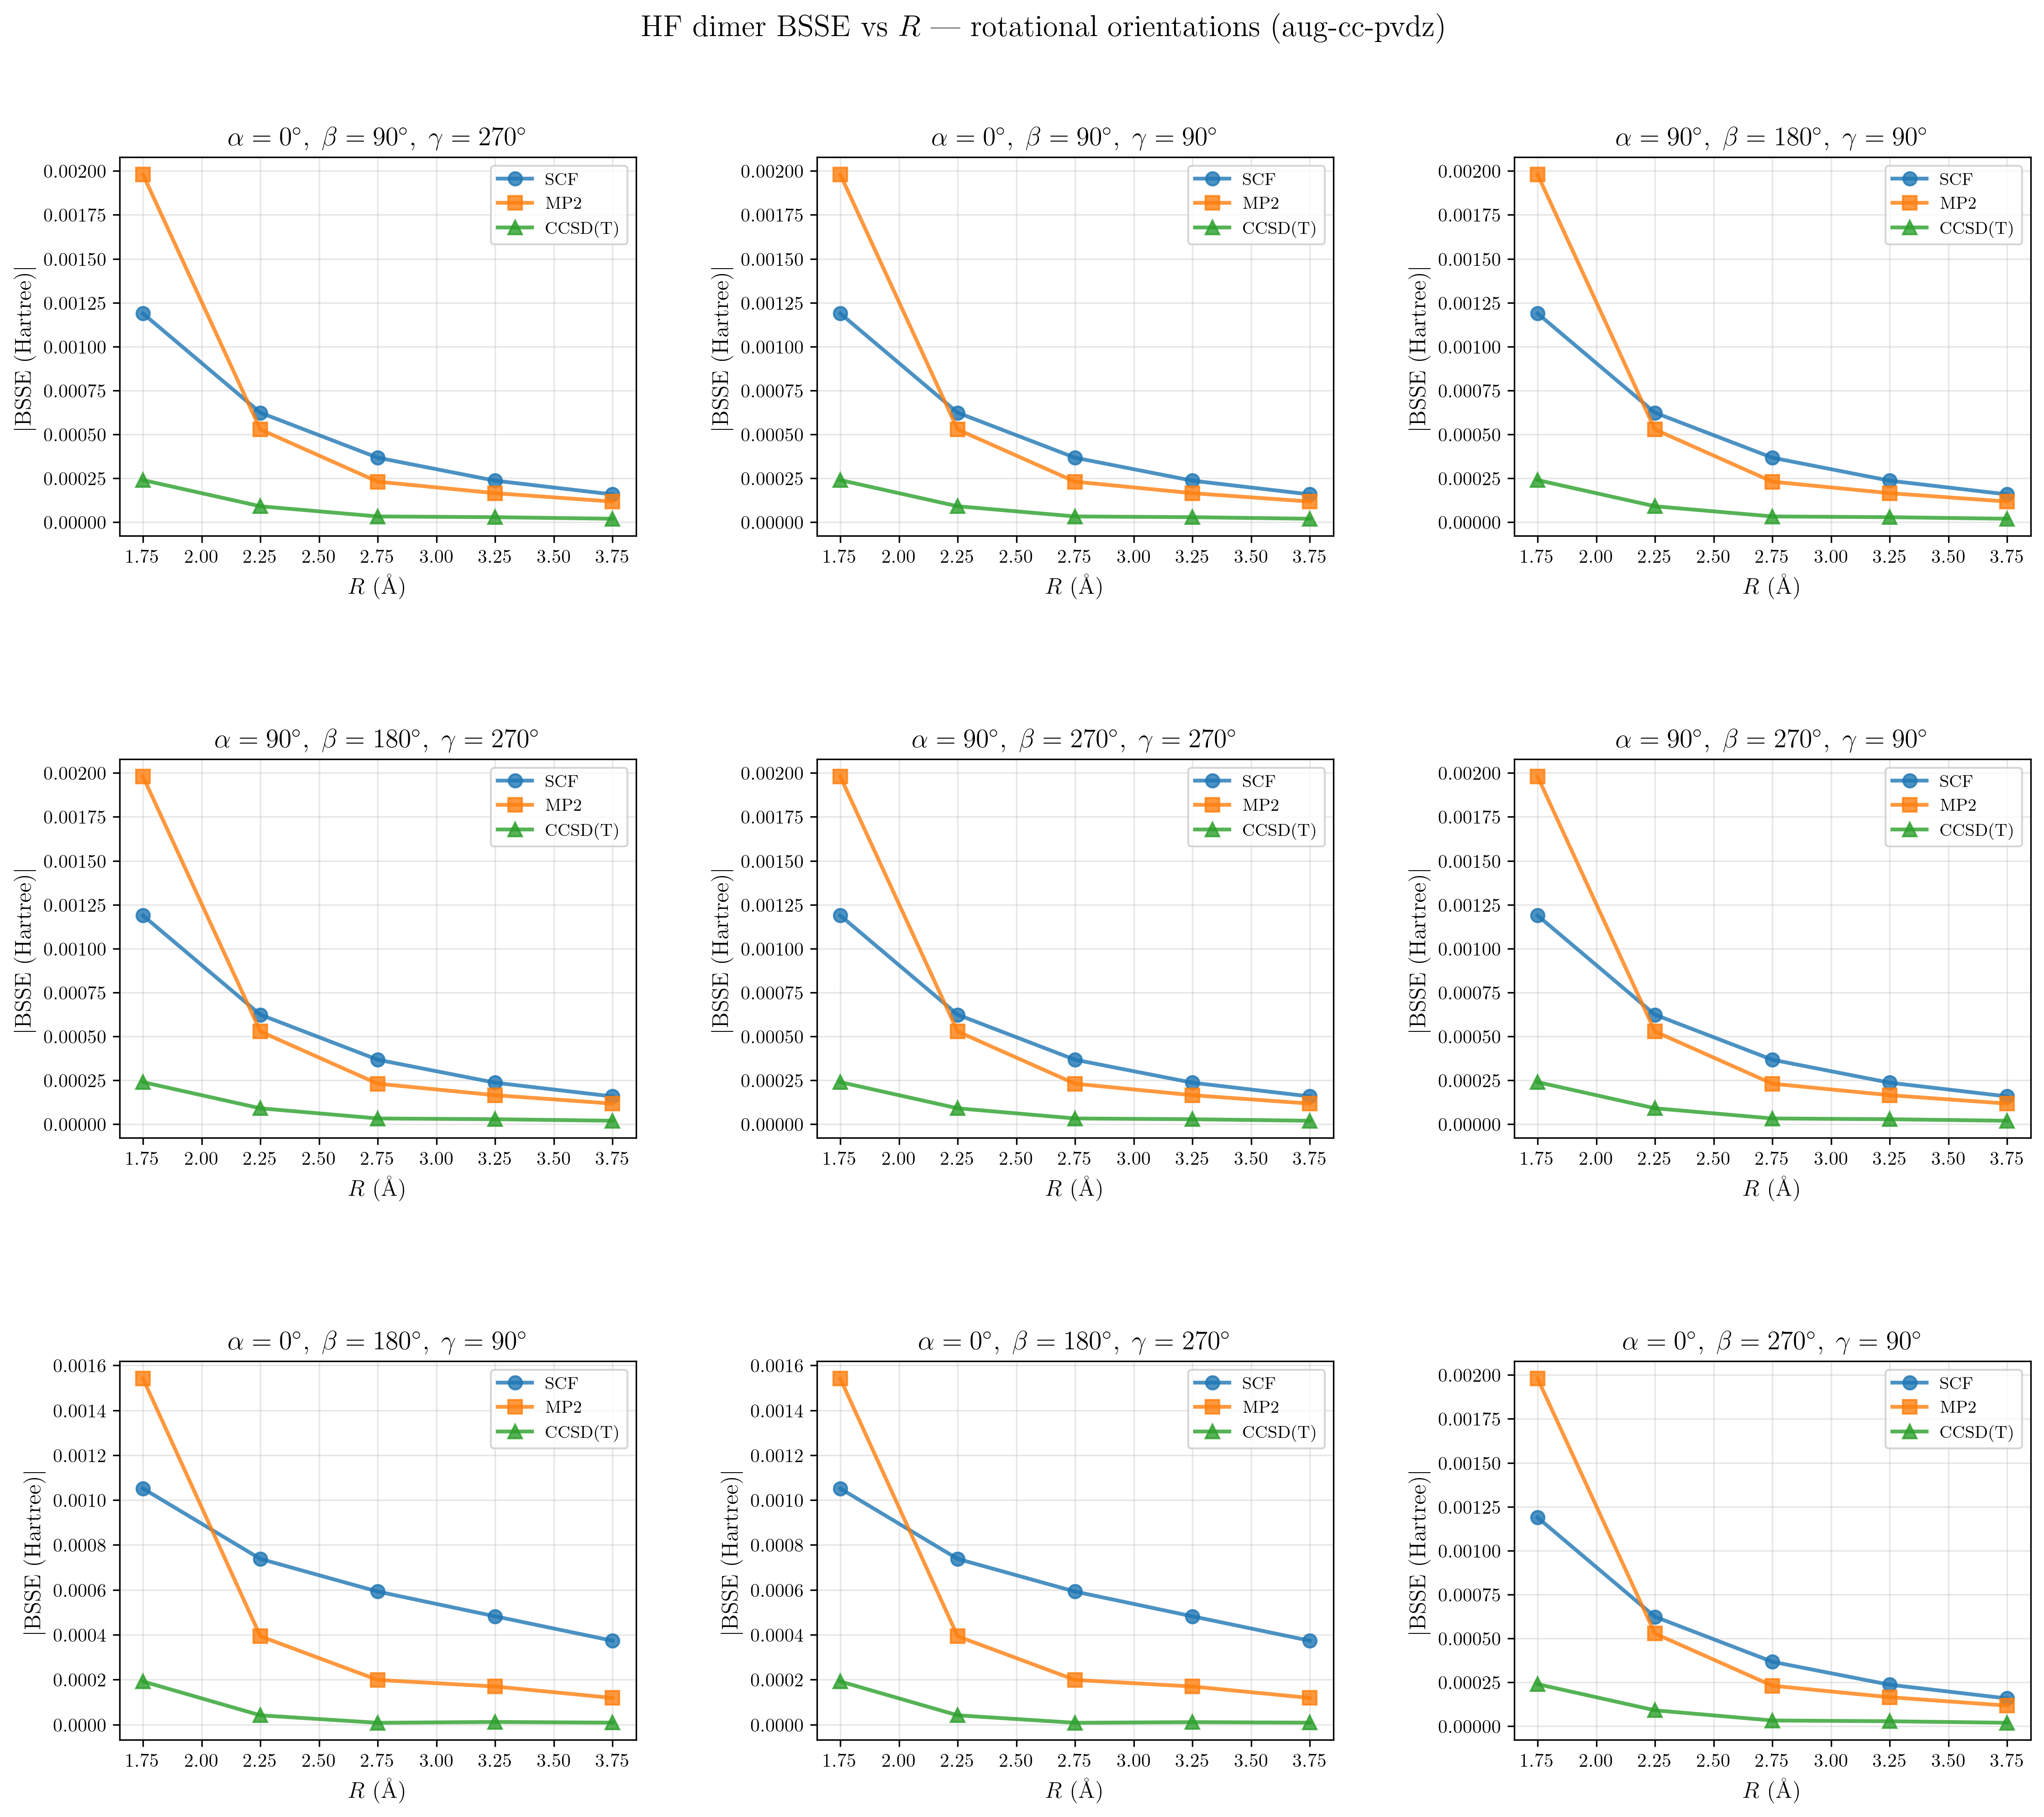
\includegraphics[scale=0.38]{figures/dimer/HF_dimer/HF_rot_vs_R_SCFMP2CCSD_T.png}
    \caption{$|\text{BSSE}|$ vs F--F separation $R$ for 9
    representative rotational orientations of the HF dimer at the
    aug-cc-pVDZ level. Each panel corresponds to a distinct set of
    Euler angles $(\alpha, \beta, \gamma)$ as labeled; all orientations
    have $\alpha = 90.0°$. Blue circles: SCF contribution; orange
    squares: MP2 correlation component
    ($E_\text{MP2} - E_\text{SCF}$); green triangles: CCSD(T)
    correlation component ($E_{\text{CCSD(T)}} - E_\text{MP2}$).
    All three components decay monotonically with $R$ and show
    consistent behavior across orientations, confirming weak
    orientation dependence of HF dimer BSSE despite the asymmetry
    observed in the SCF translational contours.}
    \label{fig:hf_rot_bsse_vs_R}
\end{figure}

\clearpage

All 9 orientations show identical monotonic decay of $|\text{BSSE}|$
with $R$ across all three methods. The shape and magnitude of the
curves are consistent across the sampled $(\alpha, \beta, \gamma)$
values, confirming that the orientation dependence of HF dimer BSSE
is weak overall --- the asymmetry visible in the SCF translational
contour at $y = \SI{1.75}{\angstrom}$ does not translate into
significant variation across rotational orientations at fixed $R$.
As in the Ne and \ce{H2O} dimers, the MP2 correlation component is
the dominant contribution at all distances sampled.



% ----------------------------------------------------------------------
\subsection{Key Findings}
% ----------------------------------------------------------------------

\begin{finding_box}
\textbf{HF dimer BSSE is primarily governed by F--F distance, with a
physically real short-range asymmetry.}
The translational contour plots show nearly circular arcs at
$y = \SI{1.5}{\angstrom}$, consistent with Ne and \ce{H2O}. At
$y = \SI{1.75}{\angstrom}$, the SCF contours develop a visible
asymmetry between the $x$ and $z$ directions. This asymmetry is
confirmed to be a physical effect of the heteronuclear HF geometry:
at short range, when the displacement components are comparable to
the HF bond length, the orientation of H vs F becomes observable in
the SCF BSSE. The MP2 and CCSD(T) correlation components remain
circular at both $y$ values.
\end{finding_box}

\begin{finding_box}
\textbf{Orientation dependence of HF dimer BSSE is weak overall.}
Despite the asymmetry in the SCF translational contours, the
rotational--radial scan shows that $|\text{BSSE}|$ vs $R$ curves are
consistent across all 28 eligible orientations. The dominant
contribution across all distances and orientations is the MP2
correlation component, with a small CCSD(T) increment, mirroring the
behavior seen in the Ne and \ce{H2O} dimers.
\end{finding_box}

\clearpage